\documentclass[a4paper,12pt,twoside]{proyectotanquesecci}
\usepackage{graphicx}
\usepackage{eqparbox}
\usepackage[tight,footnotesize]{subfigure}
\usepackage{hyperref}
\usepackage[spanish]{babel}
\selectlanguage{spanish} 
\usepackage[utf8]{inputenc}
\hyphenation{op-tical net-works semi-conduc-tor}
\usepackage{algpseudocode}
\usepackage{algorithm}
\usepackage{colortbl}
\usepackage{fancyhdr}
\usepackage{anysize}
\marginsize{3cm}{3cm}{2.5cm}{2.5cm}
\title
{
\textbf{Capítulo de libro del grupo de control (M-ECCI)}\\
\vspace{3cm}
{\large 
Dayanis Andrea Suarez Rodriguez\\
Sergio Andres Acosta Herrera \\
David Humberto Hernandez Balcazar\\}
\vspace{1cm}
\textbf{Director}\\
{\large Ing. Jhon Fredy Bayona Navarro M.Sc.}\\
\vspace{2cm}
{\large Bogotá D.C.}
}
\pagestyle{fancy}
\renewcommand{\chaptermark}[1]{\markboth{#1}{}}
\renewcommand{\sectionmark}[1]{\markright{#1}}
\fancyhf{}
\lhead[\small{\thepage}]%
      {\small{\rightmark}}
\rhead[\small{\leftmark}]%
      {\small{\thepage}}
\cfoot{}
\lfoot[\small{M-ECCI}]%
      {\small{Trabajo de Grado}}
\rfoot[\small{Trabajo de Grado}]%
      {\small{M-ECCI}}
\begin{document}
\maketitle
\renewcommand{\contentsname}{Tabla de Contenido}
%\renewcommand{\listtablename}{Lista de Tablas}
\renewcommand{\listfigurename}{Lista de Figuras}
\tableofcontents
%\listoftables
\listoffigures






% ==============================================================================================
%												RESUMEN
% ==============================================================================================

\chapter*{Resumen}
\addcontentsline{toc}{chapter}{Resumen}

El presente documento describe el análisis y diseño de un prototipo de sistema de tanques acoplados al cual se aplican técnicas de control. El sistema es desarrollado teniendo en cuenta aspectos de seguridad, estándares industriales y parámetros multidisciplinarios requeridos para un módulo de laboratorio. \\

Se muestran fundamentos teóricos básicos de la lógica de control, así como de diseño para un prototipo de sistema de entrenamiento para el control de nivel de tanques acoplados. Proporciona procedimientos en los cuales se aplican diversas técnicas de control al sistema de entrenamiento diseñado. Además brinda los procedimientos necesarios que facilitan el diseño de controladores. Se compara el desempeño del controlador frente al sistema no controlado determinando ventajas e inconvenientes que presenta el sistema de control. \\

Finalmente se detallan las conclusiones obtenidas en el desarrollo del proyecto y se brindan recomendaciones para la obtención de mejores resultados tanto para el desarrollo de prácticas de laboratorio como para la implementación del sistema de entrenamiento. \\






% ==============================================================================================
%										CAPITULO INTRODUCCIÓN
% ==============================================================================================

\chapter{Introducción}

Desde los inicios del tiempo y particularmente enmarcados dentro del contexto de procesos industriales, científicos de todo el mundo han trabajado para lograr que los procesos de manufactura, control automático y accionamiento sean cada vez más efectivos y más eficientes. Con esta meta se han desarrollado nuevos procesos para lograr alcanzar este mejoramiento continuo de un sistema hidráulico para proyectos con manipulación de líquidos.\\

El diseño de los sistemas hidráulicos se basa en la interconexión de  sistemas mecánicos a través de bombas, válvulas y pistones móviles, que ofrecen una automatización factible  en el sistema. La utilidad de estos mecanismos hace que sea  funcional y  opere de una manera  eficaz básicamente para generar distintas aplicaciones de procesos industriales, sin embargo el uso es producir energías limpias mediante recursos naturales.\\

Con mayor eficiencia el nivel de tecnología en la actualidad estimula los parámetros que retroalimentan y contribuyen la necesidad del ser humano con aplicaciones que avanzan a gran escala de industria a industria de alta calidad,  los sistemas hidráulicos son construidos y desarrollados especialmente para el mejoramiento de la dinámica de fluidos como: químicos, combustible, aceites, agua, entre otros. Sin embargo estos sistemas trabajan en conjunto para realizar un análisis integral tanto dinámico, termodinámico y mecánico en el cual la particularidad de cada uno hace parte de la potencia y control de un sistema. El análisis de los mismos se realiza en un laboratorio observando el estado estable y funcional del sistema mediante una simulación computarizada.\\

La simulación se ha convertido en una herramienta fundamental para el estudio de varios sistemas técnicos. En los sistemas hidráulicos la simulación juega un papel útil, verifica que todos los mecanismos se accionen adecuadamente y no presenten fallas en el sistema real; aunque las características específicas de los sistemas hidráulicos hacen difícil utilizar software de simulación de tipo general en el estudio.\\

Con frecuencia las universidades tienen herramientas y dispositivos inteligentes para obtener un análisis de investigación y desarrollo e innovación, esto permite que el estudiante requiera habilidades prácticas y capacidades a la hora de enfrentarse con un prototipo de estudio.\\





% ==============================================================================================
%										CAPITULO JUSTIFICACIÓN
% ==============================================================================================

\chapter{Justificación}

Para comprender de mejor manera las características de las técnicas de control es importante el desarrollo de una aplicación que además de simular un proceso industrial, permita analizar distintos tipos de controladores. \\

Es por esto que se ha escogido realizar un sistema de entrenamiento para el cual se pueda diseñar un sistema de control puesto que los laboratorios de la universidad no poseen módulos de ese tipo, que permitan simular procesos industriales con interacción de fluidos. \\

\section{Estado del arte}



Actualmente, la Universidad Escuela Colombiana de Carreras Industriales (ECCI) cuenta con espacios destinados para la realización de actividades prácticas en las asignaturas de Automatización, Neumática, Mecánica e Instrumentación Electrónica. Sin embargo, las actuales condiciones de los laboratorios no son suficientes para desarrollar de manera satisfactoria todas las sesiones de laboratorio, principalmente debido a no contar con una dotación de equipos actualizada, operativa y funcional para implementar nuevas practicas, ínter-disciplinarias y mas ampliamente enfocadas a pre-grados, postgrados y maestrías. La historia reciente del Laboratorio de Control de la E3T se remonta al año 2001, donde a través de un trabajo de grado denominado “Planeación, diseño y realización del laboratorio de instrumentación electrónica para la E3T” [1], se realizó el diseño, construcción, e implementación de bancos de trabajo para medición de nivel, temperatura, caudal y presión, con guías prácticas de laboratorio asociadas. \\

De otro lado, los sistemas de nivel de líquido representan un ejemplo concreto de sistema de control con amplia difusión en medios industriales. Todo proceso que necesite almacenar sustancias en estado liquido requiere realizar registros sobre el nivel de depósito de las mismas. Algunos de los sectores en los que es de gran importancia mantener el nivel de líquido entre parámetros previamente establecidos son, entre otros: la industria petroquímica, la producción de papel, el tratamiento de aguas y los procesos químicos, en los que por el grado de riesgo por contacto humano se requieren procedimientos automatizados. \\

Respecto a soluciones didácticas para sistemas de nivel de líquido, se destaca el sistema de laboratorio virtual desarrollado en la Universidad de Murcia en España en el cual se propone un sistema de tres tanques acoplados con acceso remoto vía Internet [3]. También en [4] se implementa el diseño y la instrumentación de un sistema de tanques acoplados para prácticas de laboratorio universitario. En [5] se aplica un control predictivo para mantener el nivel de líquido en un prototipo de proceso industrial. En Colombia se destacan algunos trabajos, entre ellos [6] de la UPB-Medellin donde se plantea una solución para la industria de tintorerías local a partir de un control de nivel y [7] de UNAL-Manizales donde se diseña un sistema automatizado de control de nivel para la industria de lácteos en el eje cafetero. En la Universidad Industrial de Santander se han desarrollado varios proyectos de grado relacionados con el control y la automatización de sistemas de nivel de liquido, entre ellos se destacan [8, 9, 10]. \\





% ==============================================================================================
%										CAPITULO OBJETIVOS
% ==============================================================================================

\chapter{Objetivos}

\section{Objetivo general}

\begin{enumerate}
\item Diseñar un sistema de control de un sistema de entrenamiento para control de nivel de líquidos de tanques acoplados.
\end{enumerate}

\section{Objetivos específicos}

\begin{enumerate}
\item Obtener el modelo matemático para la respuesta del nivel del sistema.
\item Diseñar un controlador que permita mantener el nivel del sistema en el set-point establecido por el usuario.
\item Evaluar el comportamiento dinámico del nivel en la planta, de acuerdo al flujo de entrada.
\end{enumerate}





% ==============================================================================================
%										CAPITULO MARCO TEORICO
% ==============================================================================================

\chapter{Marco Teórico}

\section{Introducción a Sistemas hidráulicos}

Un sistema hidráulico es uno en el cual los líquidos, generalmente son considerados flujo incomprensible. Los sistemas hidráulicos comúnmente aparecen en procesos químicos, sistemas de control automático; y actuadores y motores de accionamiento para la fabricación de equipos. Estos sistemas son usualmente interconectados a sistemas mecánicos a través de bombas, válvulas, y pistones móviles. Una turbina es impulsada por agua y usada para accionar un generador eléctrico es un ejemplo de un sistema donde interactúan elementos hidráulicos, mecánicos y eléctricos. No discutiremos más sobre el tema general de sistemas fluidos, el cual podría incluir fluidos compresibles tales como gases y aire. \\

Un análisis exacto de sistemas hidráulicos no es usualmente factible por su naturaleza distribuida y el carácter no lineal de la resistencia al flujo. Para nuestro análisis dinámico, sin embargo, podemos obtener resultados satisfactorios debido al uso de elementos agrupados y linealizando los resultados no lineales de modelos matemáticos. Por otra parte el diseño de procesos químicos requiere un análisis más exacto donde los modelos estáticos son usados más que los dinámicos.\\

En más casos, los sistemas hidráulicos operan con las variables restantes cerca de un punto de operación específico. Generalmente estamos interesados en los modelos que involucran variables incrementales. Este hecho es particularmente útil porque tales modelos son usualmente lineales, aunque el modelo expresado en las variables finales podría ser no lineal.\\

\newpage





% ==================================== SECCIÓN MODELAMIENTO ====================================


\section{Modelamiento}

Un modelo matemático es simplemente una imitación de la realidad, con el cual se busca usualmente ganar perspicacia sobre el comportamiento de sistemas, probándolos, controlándolos u optimizándolos. En el proceso de construcción de modelos, el principal objetivo es dar una equivalencia matemática a un problema de la vida real para luego resolver y finalmente interpretar. En los problemas de ingeniería, se busca capturar esto en forma de ecuaciones, haciendo énfasis en aspectos específicos y omitiendo aquellos que aunque hagan parte de la realidad, su contribución en ella sea mínima para simplificar el modelo y su solución. \\

\subsection{Variables}

Ya que los sistemas hidráulicos involucran el flujo  y la acumulación del líquido, las variables usadas a describir su comportamiento dinámico son:\\

\textit{w}, Velocidad del flujo en metros cúbicos por segundo.\\ 

\textit{v}, Volumen en metros cúbicos.\\ 

\textit{h}, Altura del líquido en metros.\\ 

\textit{p}, Presión en newton por metro cuadrado.\\

A menos que se indique lo contrario, una presión será la presión absoluta. Además,  algunas veces se encontrará conveniente expresar las presiones en términos de presiones manométricas. Una presión manométrica, que se denota por $p^{*}$, se define como la diferencia entre la presión absoluta y la presión atmosférica ${p_{a}}$:

\begin{equation}
p^{*}*(t)=p(t)-pa
\label{Ecu 1}
\end{equation}

Una diferencia de presión, denotado por $\Delta p$, es la diferencia entre las presiones en dos puntos. \\

\subsection{Leyes de los Elementos}

Los sistemas hidráulicos presentan tres características típicas que pueden ser aproximadas por este grupo de elementos: capacidad, resistencia de flujo, e inertancia. En esta sección se discutiran los dos primeros. La inertancia, que representa la energía cinética de una corriente de fluido en movimiento, suele ser insignificante, y no la consideraremos.\\

\subsection{Capacitancia}

Cuando un liquido está almacenado en un recipiente abierto, existe una relación algebraica entre el volumen del líquido la presión de la base del recipiente. Si el área de la sección transversal del recipiente es dada por una función \textit{A(h)}, donde $h$ es la altura del nivel de líquido por encima del fondo del recipiente, el volumen líquido $v$ es la integral del área desde la base del recipiente a la parte superior del líquido. 
Por lo tanto,

\begin{equation}
v=\int \limits_{0}^{h} A{\lambda}d{\lambda}
\label{Ecu 2}
\end{equation}

Donde ${\lambda}$ es una variable ficticia de integración. Para un líquido de densidad $p$ expresada en kilogramos por metro cúbico, la presión \textit{p} absoluta y la altura del líquido \textit{h} están relacionadas por:

\begin{equation}
p=pgh+p_{a}
\label{Ecu 3}
\end{equation}

Donde \textit{g} es la constante gravitacional ${9.807 m/s^{2}}$ y donde \textit{Pa} es la presión atmosférica, que ha sido tomada como ${1.013 x 10^{5}  N/m^{2}}$\\

\begin{equation}
C=\frac{A}{pg}
\label{Ecu 4}
\end{equation}

Las ecuaciones (2.2) y (2.3) implican que para cualquier geometría del recipiente, la densidad del líquido y la presión atmosférica, tienen una relación algebraica única entre la presión \textit{p} y el volumen de líquido \textit{v}. Una curva característica típica que describe esta relación se muestra es la Figura 4.1.


\begin{figure}[h]
\centering
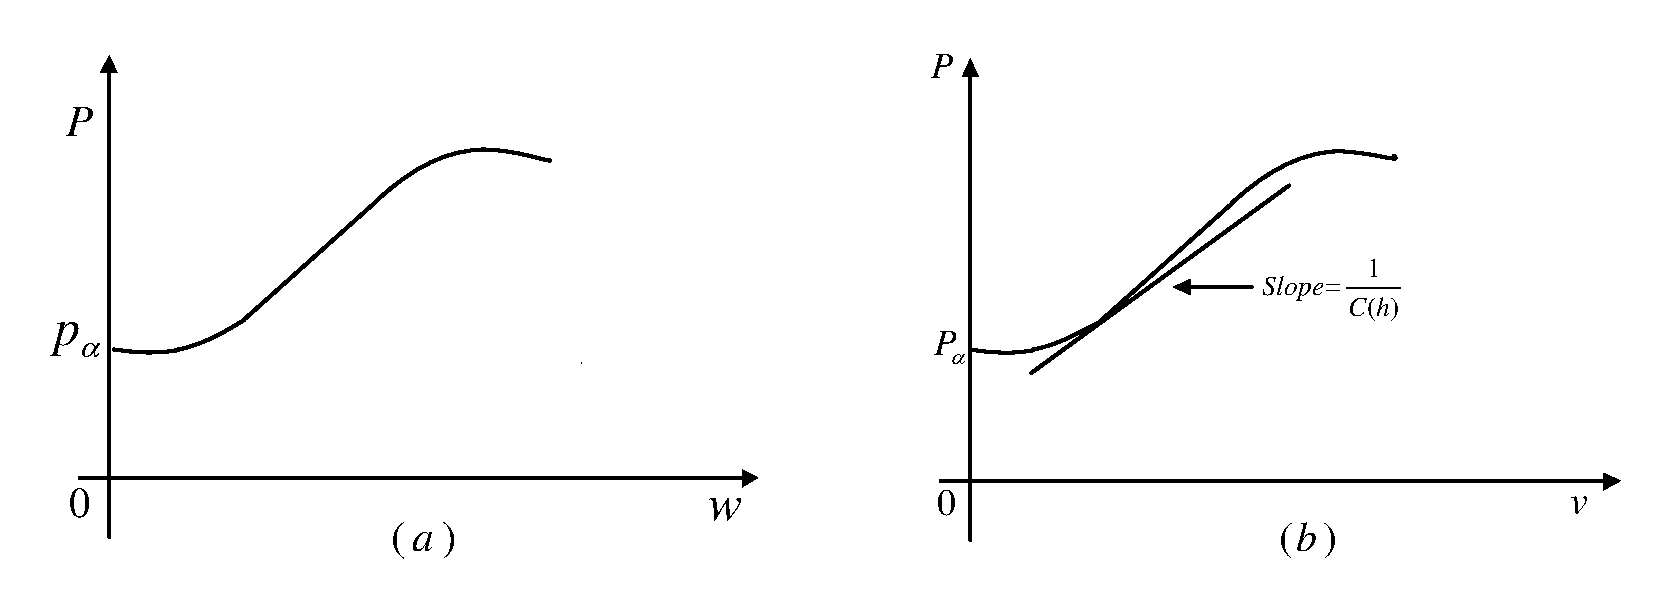
\includegraphics[scale=0.4]{Figura1}
\renewcommand{\figurename}{Fig.}
\caption{Presión en función del volumen y el área de un liquido}
\label{Presión en función del volumen y el área de un liquido}
\end{figure}

Si la tangente para la curva  presión vs volumen es dibujada en algún punto, como se muestra en la figura 1 (b), entonces el recíproco de la pendiente es definido como la capacitancia hidráulica, expresada como \textit{C(h)}.\\

\begin{equation}
C{h}=\frac{A{h}}{pg}
\label{Ecu 5}
\end{equation}

\subsubsection{Ejemplo 1:}

Considere un vaso formado por un cilindro circular de Radio \textit{R} y Largo \textit{L} que contiene un líquido de densidad \textit{p} en unidades de kilogramo por metro cubico. Encuentre la capacitancia hidráulica del vaso cuando el cilindro es vertical, como se ve en la figura 2a. También evalúe la capacitancia cuando el cilindro esta sobre uno de sus lados, como se ve en la Figura 4.2(b).

\begin{figure}[h]
\centering
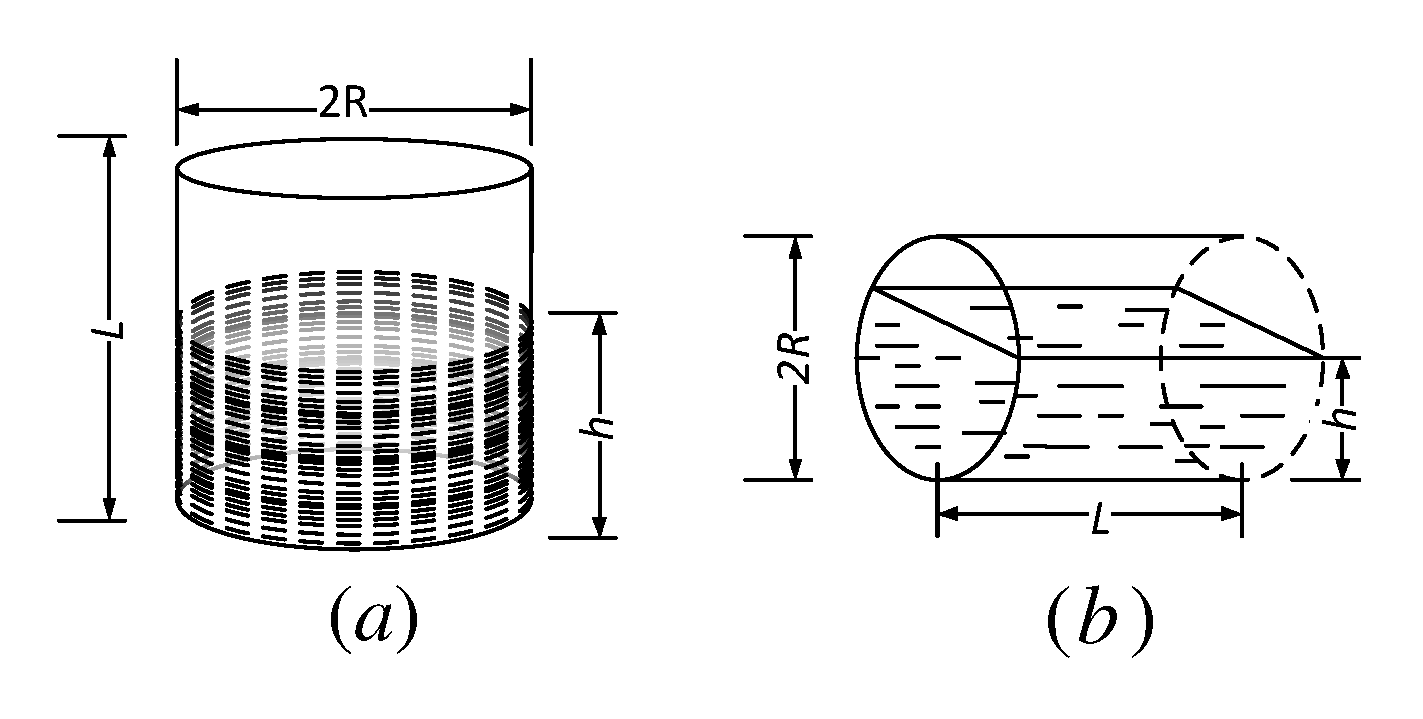
\includegraphics[scale=0.4]{Figura2}
\renewcommand{\figurename}{Fig.}
\caption{Vaso cilíndrico. (a) Vertical. (b) Horizontal.}
\label{Vaso cilíndrico. (a) Cilindro vertical. (b) Cilindro horizontal.}
\end{figure}

\subsubsection{Solución}

Para la configuración en la \textit{Fig. 4.2(a)}. El área de la sección transversal es ${\pi R^{2}}$ y es independiente de la altura del líquido. Así que se puede usar $C=\frac{A}{pg}$, y la capacitancia hidráulica del recipiente es $C_{a}=\pi\frac{R^{2}}{pg}$ \\

Cuando el recipiente esta sobre uno de sus lados, como se muestra en la Figura 4.2(b), el área de la sección transversal es una función de la altura del liquido h. Puede verificar que el ancho de la superficie del líquido es $2\sqrt{(R^{2})}-(R-h)^{2}$ la cual es cero cuando \textit{h=0} y \textit{h=2R} y tiene el máximo valor de \textit{2R} cuando \textit{h=R}. usando $C{h}=\frac{A{h}}{pg}$, encontramos que la capacitancia es:

\begin{equation}
c_{b}=\frac{2L}{pg}\sqrt{R^{2}}-(R-h)^{2}
\label{Ecu 4}
\end{equation}

Como se muestra en la figura 3.

\begin{figure}[h]
\centering
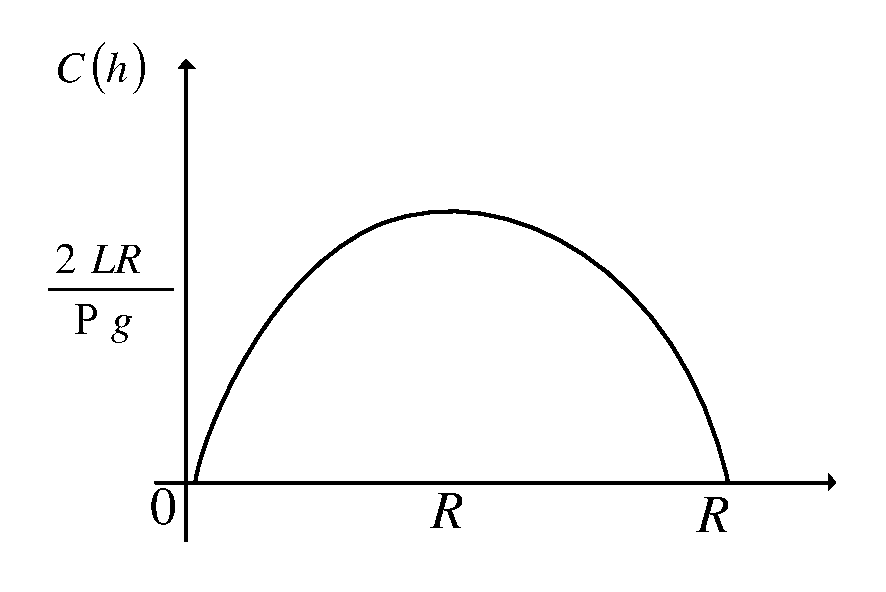
\includegraphics[scale=0.5]{Figura3}
\renewcommand{\figurename}{Fig.}
\caption{Capacitancia del recipiente.}
\label{Capacitancia del recipiente.}
\end{figure}

\subsection{Resistencia}

Como el liquido fluye a través de una tubería, allí hay poca presión del líquido a lo largo de la tubería. Del mismo modo hay poca presión si el líquido fluye a través de una válvula o en un orificio. En cambio la presión asociada con el flujo del líquido que resulta la disipación de energía y usualmente obedece a una relación algebraica no lineal entre la velocidad del flujo $\omega$ y la diferencia de presión $\Delta p$. El símbolo de la válvula se muestra en la figura 4. Esto también puede ser usado por otros elementos que disipan energía. \\

Un valor positivo de $\omega$ indica que el líquido está fluyendo en la dirección de la flecha; un valor positivo de $\Delta p$ (presión diferencial) indica que la presión en el punto marcado con $+$ es más alta que la presión en el otro punto. La expresión:

\begin{equation}
w=k\sqrt{\Delta p}
\label{Ecu 7}
\end{equation}

\begin{figure}[h]
\centering
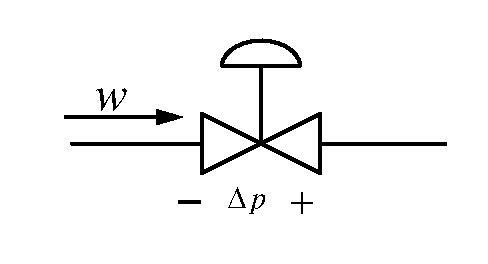
\includegraphics[scale=0.5]{Figura4}
\renewcommand{\figurename}{Fig.}
\caption{simbolo de una válvula hidráulica.}
\label{simbolo de una válvula hidráulica.}
\end{figure}

Describe un orificio y una válvula y es una buena aproximación del flujo turbulento a través de las tuberías. Se pueden tratar todas las situaciones que sean de interés, usando una ley de un elemento no lineal de la forma de (7). En esta ecuación, $k$ es una constante que depende de las características de la tubería, válvula, u orificio. Una curva típica de la velocidad del flujo contra la presión diferencial como se muestra en la \textit{Fig. 2.5(a)}.

\begin{figure}[h]
\centering
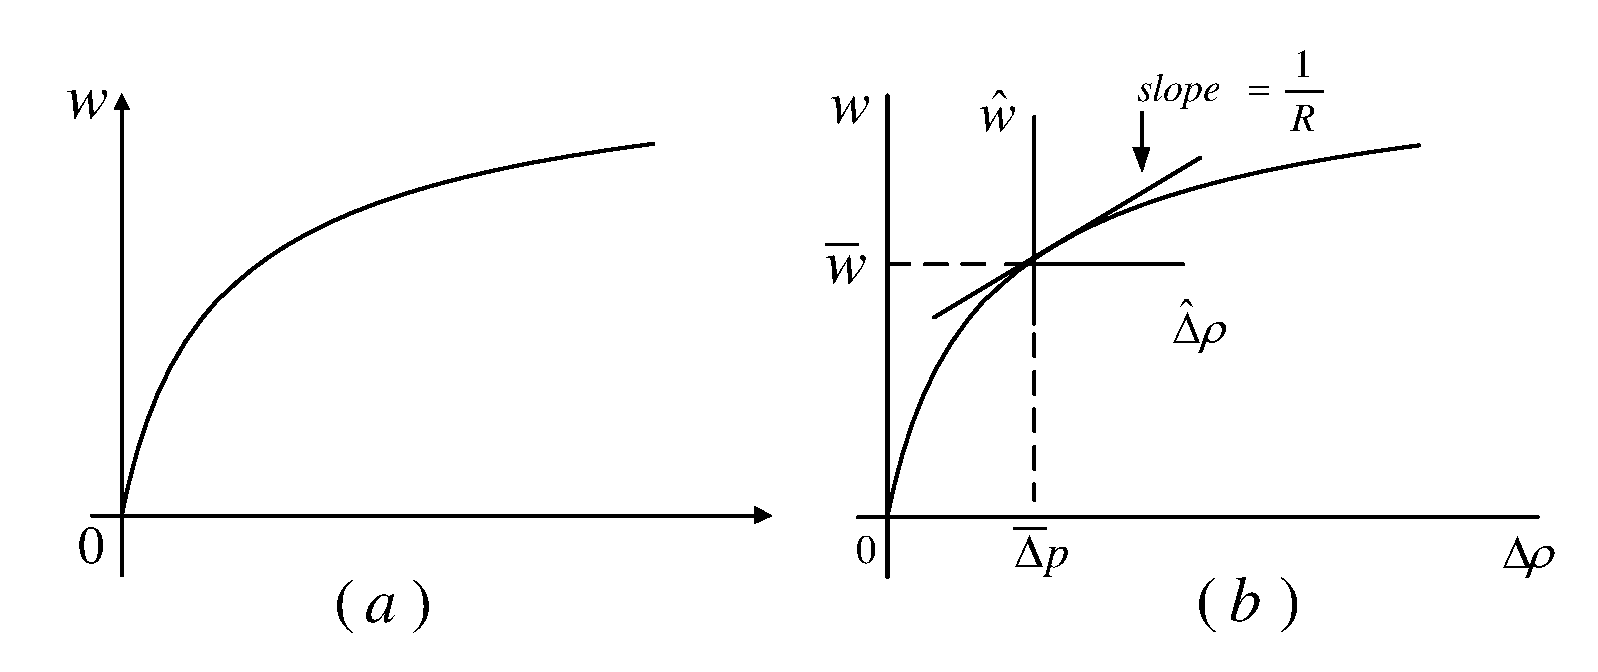
\includegraphics[scale=0.5]{Figura5}
\renewcommand{\figurename}{Fig.}
\caption{(a) velocidad de flujo vs presión diferencial. (b) Interpretación de la resistencia hidráulica.}
\label{(a) velocidad de flujo vs presión diferencial. (b) Interpretación de la resistencia hidráulica.}
\end{figure}

Ya que (7) es una relación no lineal, se debe linealizar alrededor un punto de operación a fin de desarrollar un modelo lineal de un sistema hidráulico.
Si se dibuja la tangente a la curva de $w$ verus $\Delta p$  en el punto de operación, el reciproco de su pendiente es definido como la resistencia hidráulica $R$. \\

La \textit{Fig. 5(b)} ilustra la interpretación geométrica de la resistencia, la cual tiene unidades de newton-segundos por metro.\\

Expandiendo (7) en la serie de Taylor alrededor del punto de operación dado.

\begin{equation}
w=-w+\frac{dw}{d\Delta p}\downarrow -\Delta p (\Delta p -\Delta p - ....)
\end{equation}

La variable incremental $\overline{w}$  y $\overline{\Delta p}$ son definidos por:

\begin{equation}
\widehat{w}=w-\overline{w}
\end{equation}

\begin{equation}
\overline{\Delta p}=\Delta p - \overline{\Delta p} 
\end{equation}

Y el segundo y primer término en la expansión son descartados. Así el modelo incremental se convierte

\begin{equation}
\widehat{w}=\frac{1}{R}-\overline{\Delta p}
\end{equation}

Donde

\begin{equation}
\frac{1}{R}=\frac{dw}{d\Delta p}\downarrow\overline{\Delta p}
\end{equation}

Podemos también expresar la resistencia R en términos de $\overline{\Delta p}$ ó $\overline{w}$llevarlo a la diferenciación requerida usando (10). Específicamente,

\begin{equation}
\frac{1}{R}=\frac{d}{d\Delta p}(k\Delta p_{\frac{1}{2}})\vdots \overline{\Delta p}
\end{equation}

Entonces

\begin{equation}
R=\frac{k}{2\sqrt{\Delta p}}
\end{equation} 
Para expresar la resistencia en términos de $\overline{w}$, se observa de (10) que 
\begin{equation}
\overline{w}=k\sqrt{\overline{\Delta p}}
\end{equation}

Sustituyendo (1.12) en (1.13) dada la ecuación alternativa por resistencia hidráulica como.

\begin{equation}
R=\\frac{2\overline{w}}{k^{2}}
\end{equation}

Ya que los líquidos típicamente fluyen a través de redes compuestas de tuberías, válvulas y orificios, con frecuencia se debe combinar varias relaciones de la forma de (7) en una sola expresión equivalente. Usamos los modelos linealizados en muchos de nuestros análisis de los sistemas hidráulicos, es importante desarrollar reglas para combinar las resistencias de elementos linealizados que estén en configuración serie y paralelo. En el siguiente ejemplo, considere la relación del flujo versus la presión diferencial y la resistencia equivalente para dos válvulas en serie. La situación del flujo paralelo es tratada en uno de los problemas al final del capítulo. \\

\subsubsection{Ejemplo 2:}

En la \textit{Fig. 2.6(a)}. Se muestra una configuración en serie de dos válvulas a través de las cuales fluye un líquido con una velocidad $w$ y a través del cual la presión diferencial es ${\Delta p}$, una válvula equivalente se muestra \textit{Fig. 2.5(b)}. Las dos válvulas son.

\begin{figure}[h]
\centering
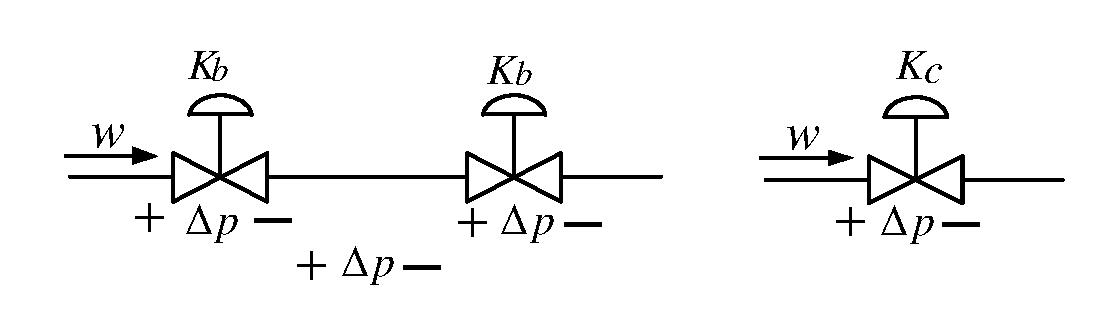
\includegraphics[scale=0.5]{Figura6}
\renewcommand{\figurename}{Fig.}
\caption{Dos válvulas en serie (b). Válvula equivalente.}
\label{Dos válvulas en serie (b). Válvula equivalente.}
\end{figure}

\subsubsection{Solución:}

Ya que las dos válvulas son conectadas en serie, tienen la misma velocidad de flujo $\omega$, y la presión diferencial total es $\Delta p = \Delta_{a}+\Delta_{b}$. Para determinar $k_{c}$, se escribe $\Delta p$ en términos de $\omega$ como:

\begin{equation}
\Delta p= \Delta p_{a}+\Delta p_{b} = \left(\frac{1}{k^{2}_{a}}+\frac{1}{k^{2}_{a}}\right)\omega^{2}
\end{equation} \\

Entonces al resolver para $w$ en términos de $\Delta p$. Después de algunas manipulaciones, se encuentra que:

\begin{equation}
w=\left(\frac{{k_{a}k_{b}}}{\sqrt{{k^{2}}_{a}+{k^{2}}_{b}}} \right)
\end{equation} \\

Comparando (2.16) con (7) se ve que la válvula constante equivalente es

\begin{equation}
k_{c}=\frac{k_{a} k_{b}}{\sqrt{k^{2}}a{k^{2}}b}
\end{equation}

Usando (2.15) para la resistencia de un modelo linealizado de una válvula equivalente. Se puede escribir:

\begin{equation}
R_{c}\frac{2\overline{\omega}}{k^{2}_{c}}=
2\overline{\omega}(\frac{1}{k^{2}_{a}}+\frac{1}{k^{2}_{b}})
\end{equation} \\

Sin embargo, para aplicar (2.15) a una válvula individual, se observa que estas resistencias son $R_{a}=2\overline{\omega}/k^{2}_{a}$ y $R_{b}=2\overline{\omega}/k^{2}_{b}$ respectivamente. Usando estas expresiones para $R_{a}$ y $R_{b}$, se puede reescribir como:

\begin{equation}
R_{c}=R_{a}+R_{b}
\end{equation}

La cual es idéntica al resultado para un circuito eléctrico lineal. \\

\subsection{Fuentes}

En la mayoría de los sistemas hidráulicos, la fuente de energía es una bomba que deriva su poder de un motor eléctrico. Consideraremos la bomba de tipo centrífuga moviéndose a velocidad constante, que es ampliamente utilizada en procesos químicos. La representación simbólica de una bomba se muestra en la Figura 2.7. Relaciones insumo - producto típicos para una bomba centrífuga siendo conducido a tres velocidades constantes diferentes se muestran en la figura 9. Curvas de la bomba de $\Delta p$ versus $\omega$.

\begin{figure}[h]
\centering
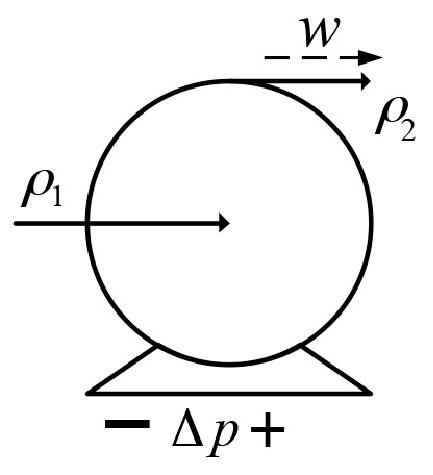
\includegraphics[scale=0.5]{Figura7}
\renewcommand{\figurename}{Fig.}
\caption{Representación simbólica de la bomba.}
\label{Representación simbólica de la bomba.}
\end{figure}

\begin{figure}[h]
\centering
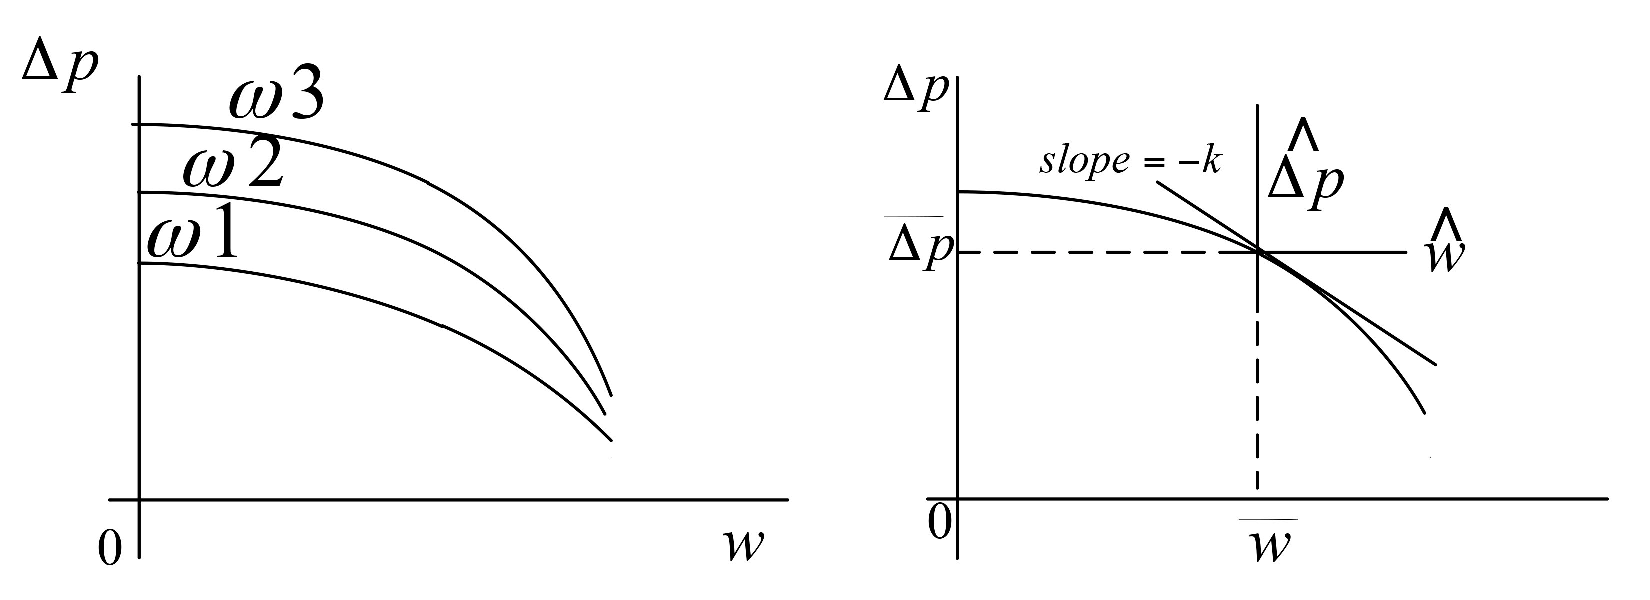
\includegraphics[scale=0.5]{Figura8}
\renewcommand{\figurename}{Fig.}
\caption{Curvas típicas de la bomba centrífuga donde $\delta p=p_{2}-p_{1}$ (a) para tres diferentes velocidades de la bomba ($\omega1 < \omega2 < \omega3$). (b) muestra la aproximación lineal.}
\label{Curvas típicas de la bomba centrífuga donde $\delta p=p_{2}-p_{1}$ (a) para tres diferentes velocidades de la bomba ($\omega1 < \omega2 < \omega3$). (b) muestra la aproximación lineal.}
\end{figure}

Se determinan experimentalmente en condiciones de estado estacionario y son bastante no lineal. Para incluir una bomba impulsada a una velocidad constante en un modelo dinámico lineal, primero se determina el punto de funcionamiento de la velocidad de la bomba en particular mediante el cálculo de los valores de \textit{p} y $\omega$. Entonces nos se encuentra la pendiente de la tangente a la curva de la bomba en el punto de trabajo y se define que sea \textit{-K}, que tiene unidades de newton-segundo por metro. Sabiendo donde está, se puede expresar la diferencia de presión gradual $p$ en términos de la tasa de flujo adicional $\omega$ como:

\begin{equation}
\Delta p=-K\widehat {\omega}
\end{equation}

Donde la constante $K$ es siempre positiva. La solución de la ecuación anterior para $\omega$ produce:

\begin{equation}
\widehat {\omega}=-\frac {1}{K}\widehat {\Delta p}
\end{equation}

Figura 9 (b) Ilustra la relación de la aproximación linealizada a la curva de la bomba no lineal. Se puede escribir la expansión de la series de Taylor para una bomba accionada a una velocidad constante como:

\begin{equation}
\omega =\overline {\omega }+\frac {d\omega }{d\Delta p} \downarrow \frac {\left( \Delta p-\overline {\Delta p}\right)}{\Delta p} +\ldots 
\end{equation}

Donde el coeficiente $\frac {d\omega }{d\Delta p} \downarrow \frac {}{\Delta p}$ esta es la pendiente de la tangente a la curva de $\omega$ versus $\Delta p$, medida en la operación punto, y tiene el valor $-\frac{1}{K}$. dejando caer los términos de la segunda y de orden superior en la expansión y el uso de las variables incrementales $\omega$ frente $\widehat{\Delta p}$, se obtiene la relación lineal de $\widehat {\omega}=-\frac {1}{K}\widehat {\Delta p}$. \\
La manera en cual una constante rápida de la bomba puede estar incorporada entre el modelo dinámico de un sistema hidráulico está ilustrado en el ejemplo 4 en la siguiente sección. \\

\subsection{Modelos Dinamicos de Sistemas Hidraulicos}

En esta sección, se aplican las leyes y técnicas de análisis de la sección previa. Se procede a desarrollar y analizar los modelos dinámicos para un solo recipiente (tanque) con una válvula y una moto-bomba. En cada caso, se deriva el modelo no lineal y luego se desarrolla y analiza un modelo linealizado. \\

\subsubsection{Ejemplo 3:}

La Figura 10. Muestra un recipiente que recibe líquido a un caudal $\omega_{i}\left(t\right)$ y pierde  líquido a través de una válvula que obliga la no linealidad de relación flujo contra presión $\omega _{0}=k\sqrt {P_{1}-P_{a}}$. El área de la sección transversal es \textit{A} y la densidad del líquido es $\rho$. \\

La derivada del modelo no lineal obliga para la presión absoluta $\rho_{1}$ al fondo del recipiente. Luego desarrollar la versión linealizada que es válida en la vecindad de la operación punto, y encontrar la función de trasferencia relacionado la transformación de la entrada incremental $\omega_{i}\left(t\right)$ y la presión incremental $\rho_{1}$.

\begin{figure}[h]
\centering
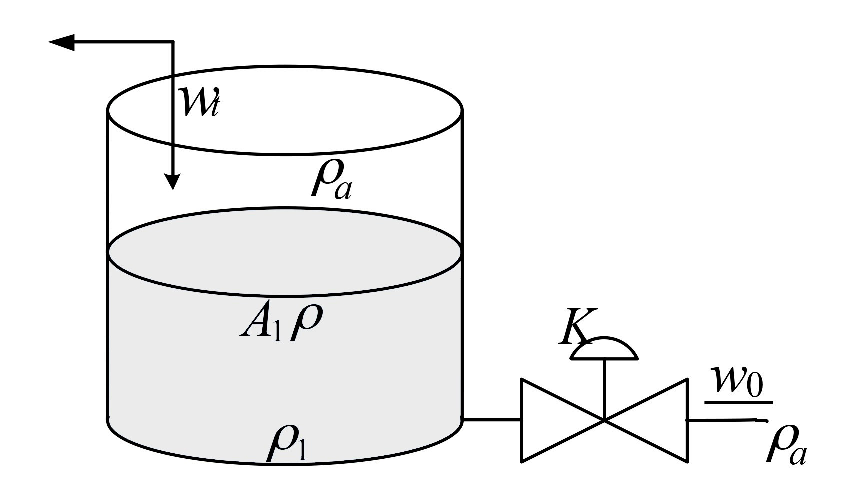
\includegraphics[scale=0.6]{Figura9}
\renewcommand{\figurename}{Fig.}
\caption{Sistema hidráulico para el ejemplo 3.}
\label{Sistema hidráulico para el ejemplo 3.}
\end{figure}

Teniendo desarrollados los modelos de sistemas en forma literal, determinar en forma numérica el punto de operación, la función de transferencia, y la respuesta a un aumento de función al paso del 10\% en el caudal de entrada para los siguientes valores de parámetros:

%\begin{equation}
\begin{center}
$A=2m^{2}$ \\
$\rho=1000\frac {k}{m^{3}}$ \\
$k=5.0\times 10^{-5}\frac {m^{4}}{s}\times N^{\frac {1}{2}}$ \\
$\overline{\omega _{i}}=6.0\times 10^{-3}\frac {m^{3}}{s}$ \\
\end{center}
%\end{equation}

\subsubsection{Solución:}

Tomando la presión $p_{1}$ como la variable de estado, utilizamos $p=\frac {1}{c}\left[ w_{in}\left( t\right) -W_{out}\left( t\right) \right]$, con $C\left(h\right)$ sustituida por la constante. $C=A/\rho g$, a escribir

\begin{equation}
p=\frac {1}{c}\left[ w_{in}\left( t\right) -W_{out}\left( t\right) \right]
\end{equation}

Luego de reemplazar y sustituir las ecuaciones para el desarrollo del planteamiento del problema se encuentra el sistema de la función de transferencia $H\left( s\right) =p_{1}\left( s\right) /w_{i}\left( s\right)$ es

\begin{equation}
H\left( s\right) =\frac {\frac {1}{C}}{s+\frac {1}{RC}}
\end{equation}

Cual tiene un solo polo en $S=-\frac{1}{RC}$. Para el valor del parámetro especificado, el punto de operación dada se reduce a

\begin{equation}
P_{1}=1.013\times 10^{5}+\left( \frac {6.0\times 10^{-3}}{5.0\times 10^{-5}}\right) ^{2}=1.157\times 10^{5}\frac {N}{m^{2}}
\end{equation}

La altura nominal del líquido es

\begin{equation}
h=\frac {1.440\times 10^{4}}{1000\times 9.807}=1.468m
\end{equation}

El valor numérico de la resistencia hidráulica y capacitancia son, respectivamente,

\begin{equation}
R=\frac {2\times 60\times 10^{-3}}{\left( 50\times 10^{-5}\right) ^{2}}=4.80\times 10^{6}N\times S/m^{5}
\end{equation}

\begin{equation}
C=\frac {20}{1000\times 9.807}=2.039\times 10^{-4}m^{5}/N
\end{equation}

Sustituyendo este valor de $R$ y $C$ entre la ecuación anterior de la función de transferencia, se puede obtener la forma numérica  de la función de transferencia como

\begin{equation}
H\left( s\right) =\frac {4904}{s+1.0216\times 10^{-3}}
\end{equation} \\

Si $\omega_{i}(s)$ es originalmente igual a este valor nominal de $\overline {w}_{i}=6.0\times 10^{-3}m^{3}/s$ y sufre un 10\% aumento paso a la función, luego $w_{i}\left( t\right) =\left[ 0.60\times 10^{-3}\right] U\left( t\right) \frac {m^{3}}{s}$ y $w_{i}\left( s\right) =\left[ 0.60\times 10^{-3}\right] \left( \frac {1}{s}\right)$. Tenemos.

\begin{equation}
P_{1}\left( s\right) =\frac {4904\times 0.60\times 10^{-3}}{s\left( s+1.0216\times 10^{-3}\right) }
=\frac {2.942}{s\left( s+1.0216\times 10^{3}\right) }
\end{equation}

Del teorema del valor final, el estado estacionario de $p_{1}$ es $p_{1}(s)$ evaluado en $s=0$, a saber

\begin{equation}
\lim _{t\rightarrow \infty }P_{1}\left( t\right) =\frac {2942}{1.0216\times 10^{-3}}=2880N/m^{2}
\end{equation}

La constante de tiempo del modelo linealizado es $\tau = RC$, cual se convierte en 

\begin{equation}
\tau =\left( 4.80\times 10^{6}\right) \left( 2.039\times 10^{-4}\right) =978.7s
\end{equation}

Que es un poco más de 16 minutos. Teniendo la respuesta que la presión incremental es

\begin{equation}
P_{1}=2888\left( 1-\in \right) \ldots falta\ldots
\end{equation}

El cambio en el nivel incremental es $\frac{p_{1}}{p}$, cual se convierte en 

\begin{equation}
h=0.2937\left( 1-\in \right) \ldots falta\ldots 
\end{equation}

Al obtener la respuesta de la presión del caudal y el nivel de líquido, nos limitamos a añadir los valores nominales $p_{1}=1.157\times 10^{5}\frac {N}{m^{2}}$ y $h=1.468m$ de las variables incrementales. Es interesante observar que a causa de la válvula no lineal, el aumento del 10\% en los resultados de la velocidad de flujo en un aumento del 20\% tanto en la presión manométrica $p_{1}-p_{a}$ y la altura $h$. \\

\subsubsection{Ejemplo 4:}

Encontrar el modelo linealizado del sistema hidráulico mostrado en la Figura 11 (a) que consiste en una bomba centrífuga de velocidad constante la alimentación de un recipiente desde el cual fluye líquido a través de una tubería y válvula de obedecer a la relación $\omega _{0}=k\sqrt {P_{1}}-P_{a}$. La característica de la bomba de la velocidad $W$ de la bomba especificada se muestra en la figura 12.11 (b). \\

\subsubsection{Solución:}

La condición equilibrada para el sistema corresponde a 

\begin{equation}
\omega _{i}=\omega _{0}
\end{equation}

Donde $\omega_{i}$ y $\Delta p=p_{1}-p_{a}$ debe ser uno de los puntos de la curva de la bomba en la Figura 11 (b), y donde $\omega_{o}$ obedece a la relación de flujo no lineal.

\begin{equation}
\omega_{o}=K\sqrt{\Delta p}
\end{equation}

Para determinar el punto de trabajo, se encuentra con la solución de $\omega_{i}=\omega_{o}$ gráficamente trazando la característica de la válvula  $\omega_{o}=K\sqrt{\Delta p}$  en la curva de la bomba. \\

Hacer esto dada la Figura 12 (a), en el que el punto de trabajo es la intersección de la curva de la válvula y la curva de la bomba, designado como punto $A$ en la figura, una vez que se ha localizado el punto de operación, se puede trazar la tangente a la curva de la bomba como se muestra en la figura 12 (b) y determinar su pendiente -K gráficamente.

\begin{figure}[h]
\centering
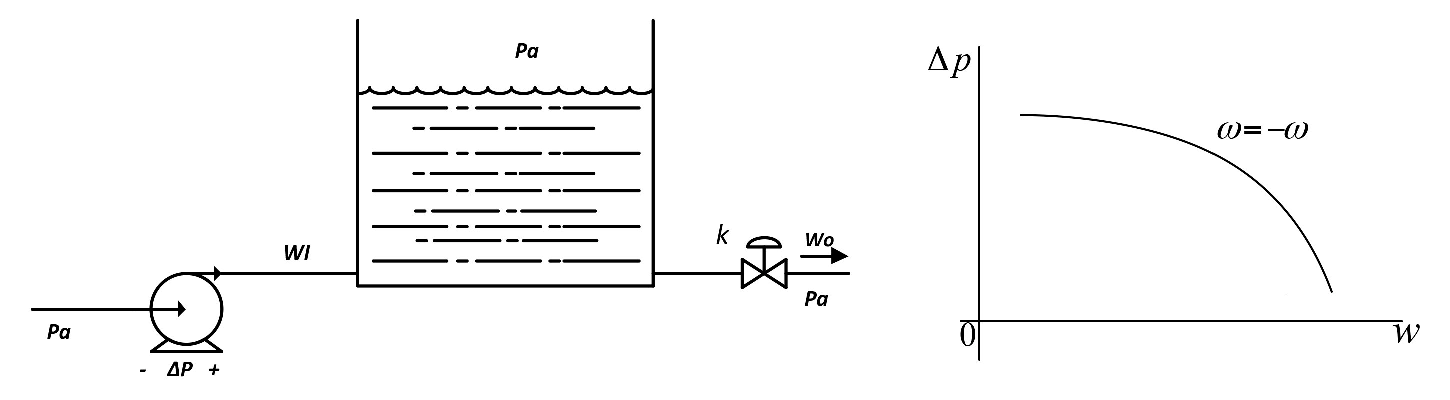
\includegraphics[scale=0.6]{Figura10}
\renewcommand{\figurename}{Fig.}
\caption{(a) Sistema para el Ejemplo 4. (b) Curva de la bomba}
\label{(a) Sistema para el Ejemplo 4. (b) Curva de la bomba}
\end{figure}

\begin{figure}[h]
\centering
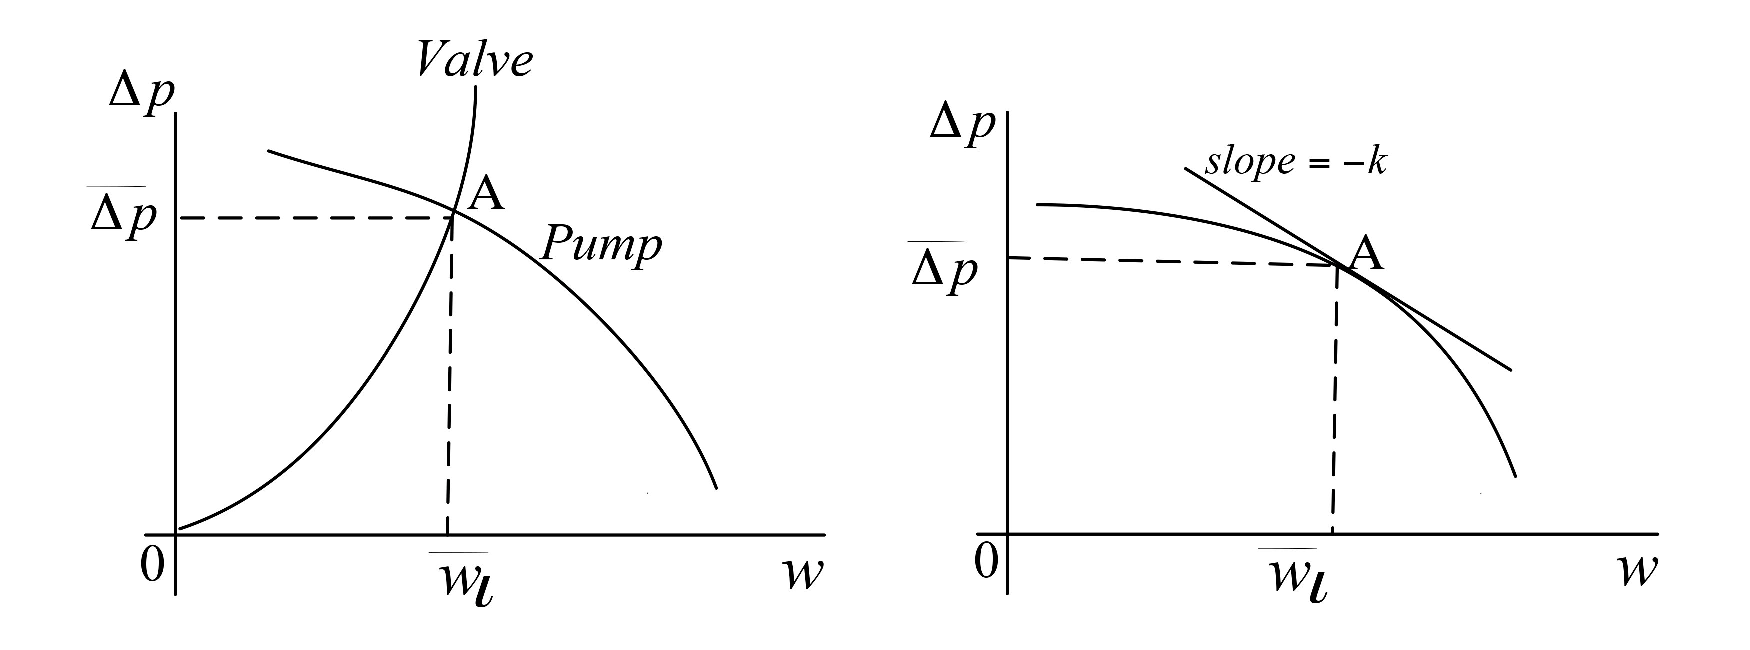
\includegraphics[scale=0.5]{Figura11}
\renewcommand{\figurename}{Fig.}
\caption{(a) Curvas de bombas y válvulas combinadas del Ejemplo 4. (b) curva de la bomba con la aproximación lineal.}
\label{(a) Curvas de bombas y válvulas combinadas del Ejemplo 4. (b) curva de la bomba con la aproximación lineal.}
\end{figure}

Después de esta etapa preliminar, se puede utilizar $p_{1}=\frac{1}{c} \left(\omega_{i}-\omega_{o}\right)$ para escribir el modelo desde el sistema como:

\begin{equation}
p_{1}=\frac{1}{c} \left(\omega_{i}-\omega_{o}\right)
\end{equation}

Donde, de $\widehat {\omega }=\frac {1}{R}\widehat {\Delta P}$, el caudal aproximado a través de la válvula es 

\begin{equation}
\omega _{0}=\overline {\omega _{0}}+\frac {1}{R}\widehat {\Delta p}
\end{equation}

Y donde, de $\widehat {\omega }=-\frac {1}{K}\widehat {\Delta p}$, el caudal aproximado a través de la bomba es

\begin{equation}
\omega _{i}=\overline {\omega }_{i}-\frac {1}{k}\widehat {\Delta \rho }
\end{equation}

Sustituyendo las ecuaciones anteriores entre el modelo del sistema, usando $p_{1}=\widehat {p_{1}}$ y $\omega_{i}=\omega_{o}$, y nada que $\widehat {\Delta p}=p_{1}$ porque $p_{a}$ es constante, se encuentra el modelo incremental es 

\begin{equation}
P_{1}=\frac {1}{c}\left( -\frac {1}{k}-\frac {1}{R}\right) P_{1}
\end{equation}

Cual se puede escribir como homogéneo de primer orden de la ecuación diferencial.

\begin{equation}
P_{1}+\frac {1}{c}\left( \frac {1}{k}+\frac {1}{R}\right) P_{1}=0
\end{equation}

La ecuación anterior indica que la magnitud de la pendiente de la curva sobre la bomba en el punto de operación  está entre la ecuación exactamente igual como la resistencia asociada con la válvula. 

Luego, si se evalúa la resistencia equivalente $R_{eq}$ se acuerda

\begin{equation}
R_{eq}=\frac {RK}{R+K}
\end{equation}

La cual fue derivada por un recipiente y una sola válvula, excepto por la ausencia de un caudal de entrada. \\

\subsubsection{Ejemplo 5:}

Las válvulas en el sistema hidráulico se muestra en la Figura 13 obedece el flujo de presión con la relación $\omega _{1}=K_{1}\sqrt {p_{1}}-P_{2}$ y $\omega _{2}=K_{2}\sqrt {p_{2}}-P_{a}$. La presión atmosférica es $p_{a}$, y las capacitancias de los tanques son $C_{1}$ y $C_{2}$. \\
Encuentre las ecuaciones que determine el punto de operación, y muestra como la curva de bomba es usada entonces. Un modelo derivado linealizado que es válido sobre el punto de operación. \\

\subsubsection{Solución:}

Porque la bomba y los dos tanques son en serie que equilibra las condiciones, se define el punto de operación para los tres caudales sean iguales $\omega_{p}$, $\omega_{1}$ y $\omega_{2}$.

\begin{figure}[h]
\centering
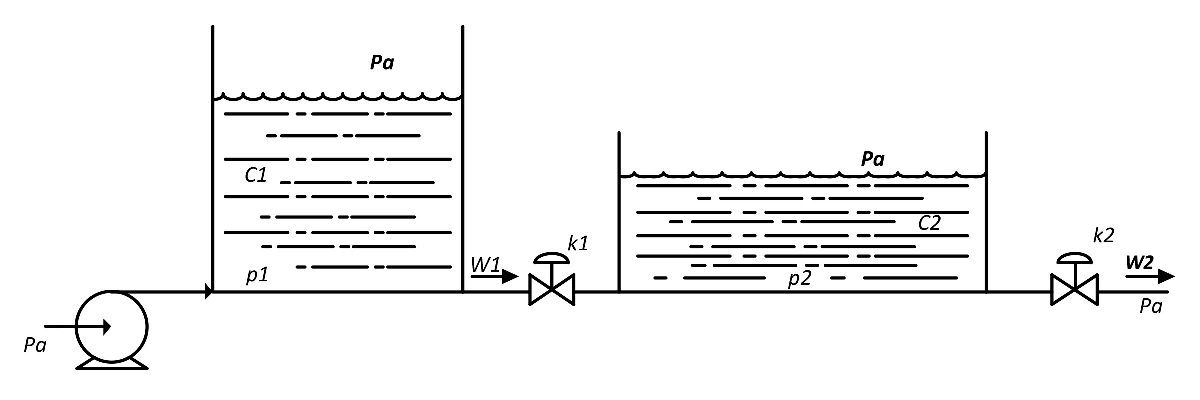
\includegraphics[scale=0.6]{Figura12}
\renewcommand{\figurename}{Fig.}
\caption{Sistema hidráulico con dos tanques considerando el Ejemplo 5.}
\label{Sistema hidráulico con dos tanques considerando el Ejemplo 5.}
\end{figure}

Los caudales a través de dos válvulas son dados por

\begin{equation}
\omega _{1}=K_{1}\sqrt {p_{1}}-P_{2}
\end{equation}

\begin{equation}
\omega _{2}=K_{2}\sqrt {p_{2}}-P_{a}
\end{equation}


El caudal $\omega_{p}$ que pasa a través de la bomba y la presión diferencial $\Delta p_{1}=p_{1}-p_{a}$ corresponde más a un punto sobre la curva de la bomba.

\begin{equation}
\omega _{p}=k_{eq}\sqrt {\Delta p_{1}}
\end{equation}

Donde,

\begin{equation}
K_{eq}=\frac {K_{1}K_{2}}{\sqrt {k^{2}_{1}}+\left( k_{2}\right) ^{2}}
\end{equation}

Graficando la ecuación anterior sobre la curva de la bomba como se muestra en la Figura 12(a) siendo las válvulas de $\Delta p_{1}$ y $\omega_{p}$, de la cual se puede encontrar otro valor nominal. \\
Con esta información, se puede desarrollar el modelo incremental. Usando $p=\frac {1}{c\left( n\right) }\left[ \omega _{in}\left( t\right) -\omega _{out}\left( t\right) \right] $,  $\omega =\frac {1}{R}\Delta p$, y $\omega =-\frac {1}{K}\Delta p$, se puede escribir el par de ecuaciones diferenciales.

\begin{equation}
p_{1}=\frac {1}{C_{1}}\left[ -\frac {1}{K}P_{1}-\frac {1}{R_{1}}\left( P_{1}-P_{2}\right) \right] 
\end{equation}

\begin{equation}
p_{1}=\frac {1}{C_{2}}\left[ -\frac {1}{R_{1}}\left( P_{1}-P_{2}\right) -\frac {1}{R_{2}}P_{2}\right] 
\end{equation}

Donde las resistencias de las válvulas son dadas por $R_{1}=\frac {2\omega _{1}}{\left( k_{1}\right) ^{2}}$ y $R_{2}=\frac {2\omega _{2}}{\left( k_{2}\right) ^{2}}$, y donde $–K$ es la pendiente de la curva de la bomba en el punto de operación. Como se indica en las ecuaciones anteriores, el modelo incremental no tiene entrada y por lo tanto puede responder solo a una condición inicial que no sea cero, que es $p_{1}(0)$ diferente de cero y/o $p_{2}$ diferente de cero. \\
En la práctica, puede haber corrientes líquidas adicionales que entran ya sea buque, o la velocidad de la bomba puede ser cambiada. También es posible para cualquiera de las dos válvulas que se abren o se cierran ligeramente. Tal cambio modificaría la respectiva resistencia hidráulica. \\
En la ausencia de una entrada, se puede transformar la ecuación anterior a encontrar la transformada de Laplace de la respuesta cero de entrada. Haciendo esto, se encuentra que después se ve:

\begin{equation}
\left[ C_{1}s+\left( \frac {1}{k}+\frac {1}{R_{1}}\right) \right] P_{1}\left( s\right) =\frac {1}{R_{1}}P_{2}\left( s\right) +C_{1}P_{1}\left( 0\right) 
\end{equation}

\begin{equation}
\left[ C_{1}s+\left( \frac {1}{R_{1}}+\frac {1}{R_{2}}\right) \right] P_{2}\left( s\right) =\frac {1}{R_{1}}P_{1}\left( s\right) +C_{2}P_{2}\left( 0\right) 
\end{equation}

Se puede encontrar cualquiera de las dos presiones $p_{1}$ o $p_{2}$ para combinarlas en estas dos ecuaciones entre una singular transformada. La correspondiente transformada inversa producirá la respuesta de entrada cero en términos $p_{1}$ y $p_{2}$. El denominador de cualquiera de las dos $p_{1}$ y $p_{2}$ estará la característica del polinomio del sistema, el cual, como se puede verificar, es:

\begin{equation}
s^{2}+\left[ \frac {1}{C_{2}}\left( \frac {1}{K}+\frac {1}{R_{1}}\right) +\frac {1}{C_{2}}\left( \frac {1}{R_{1}}+\frac {1}{R_{2}}\right) \right] s+\frac {1}{C_{1}C_{2}}\left( \frac {1}{kR_{1}}+\frac {1}{KR_{2}}+\frac {1}{R_{1}R_{2}}\right) 
\end{equation} \\

\newpage





% ==================================== SECCIÓN LINEALIZACIÓN ===================================

\section{Linealización}

Realmente, la mayoria de los sistemas fisicos de importancia practica son no lineales. La caracterización de un sistema dinamico por una función de transferencia puede ser hecha solo para sistemas lineales, aquellos descritos por ecuaciones diferenciales lineales. \\

Un sistema no lineal se define siempre y cuando no se aplique el principio de superposición, es decir, la respuesta a dos entradas no puede calcularse tomando cada una de ellas independientemente y luego sumarlas, debido a esto se usa la linealización.\\

%\begin{figure}[h]
%\centering
%\includegraphics[scale=0.5]{}
%\renewcommand{\figurename}{Fig.}
%\caption{Principio de Superposición.}
%\label{Principio de Superposición.}
%\end{figure}

La linealización es un método matemático por el cual se aproxima un sistema no lineal a uno más sencillo de analizar con una solución general del comportamiento del proceso y alrededor de un punto de operación cualquiera \textit{(xs,us)}.\\

Así pues, una función lineal es una aproximación de la función original, que se representa trazando una línea tangente al punto de operación, que se puede interpretar con la siguiente figura:\\

%\begin{figure}[h]
%\centering
%\includegraphics[scale=0.5]{}
%\renewcommand{\figurename}{Fig.}
%\caption{Punto de Operación de una función linealizada.}
%\label{Punto de Operación de una función linealizada.}
%\end{figure}

De este modo, la función linealizada solo es válida en el interior de la región representada por el círculo alrededor del punto negro en la figura 2.

%\begin{equation}
\begin{center}
	$f\left( x,u\right)=0$ \\
	$f\left( x_{s},u_{s}\right) =0$ \\
	$f\left( x,u\right) = f\left( x_{s},u_{s}\right) +\frac {\partial f}{\partial u}\left( x-x_{s}\right) +\frac {\partial f}{\partial u}\left( u+u_{s}\right) +\ldots$ \\
	$\frac {\partial f}{\partial x}\Delta x+\frac {\partial f}{\partial u}\Delta u=0$
\end{center}
%\end{equation}

\subsection{Caracteristicas de Sistemas Linealizados}

\begin{enumerate}
\item La ecuación linealizada no es única, depende del punto alrededor del cual se haya linealizado.
\item Las variables de la ecuación linealizada están dadas por incrementos con referencia al punto de operación.
\item Es más sencillo linealizar las ecuaciones término a término.
\item Diferencias de comportamiento entre el modelo linealizado y el real
\item Forma de la función a linealizar.
\item Las diferencias aumentan al alejarse del punto de equilibrio 
\end{enumerate}

\subsection{Serie de Taylor}

Para linealizar un sistema existen varios métodos tales como logaritmación, cambio de variable, series de Taylor y mínimos cuadrados, sin embargo uno muy común y el cual se utilizara en este caso son las series de Taylor, que se expresan como una suma infinita de los términos de una función.\\

Una función infinitamente derivable en un intervalo puede representarse como un polinomio a partir de sus derivadas evaluadas en un punto “a” de dicho intervalo.

%\begin{equation}
\begin{center}
	$f\left( x\right) =\sum ^{\infty }_{n=0}f^{n}\left( a\right) \frac {\left( x-a\right) ^{n}}{n!}$
\end{center}
%end{equation}

\subsubsection{Ejemplo 1:}

%\begin{equation}
\begin{center}
	$f^{0}\left( x\right) =f\left( x\right) =e^{x}$
\end{center}
%\end{equation}

\begin{enumerate}

\item Definir las derivadas de la función.
	%\begin{equation}
	\begin{center}
		$f^{1}\left( x\right) =f'\left( x\right) =e^{x}$\\
		$f^{2}\left( x\right) =f''\left( x\right) =e^{x}$\\
		$f^{3}\left( x\right) =f'''\left( x\right) =e^{x}$
	\end{center}
	%\end{equation}
\item Definir un punto de operación “a”.
	\begin{center} a=0 \end{center}
\item Definir los valores para “n” desde 0 hasta 3, hay que tener en cuenta que “n” puede llegar a valer $\infty$, sin embargo, entre mayor sea, más pequeño es el valor del termino y por tanto es despreciable para el resultado final de la ecuación. El valor de “n” también depende del número de derivaciones que pueda llegar a tener una ecuación determinada.\\

	n=0
	%\begin{equation}
	\begin{center}
		$f^{0}\left( 0\right) \frac {\left( x-0\right) ^{0}}{0!}=f^{0}\left( 0\right) \frac {1}{1}=f^{0}\left( 0\right)$\\
		$f^{0}\left( 0\right) =f\left( 0\right) =e^{0}=1$ \\
		\textit{ Primer término de la serie }\\
	\end{center}
	%\end{equation}
	
	n=1
	%\begin{equation}
	\begin{center}
		$f^{1}\left( 0\right) \frac {\left( x-0\right) ^{1}}{1!}=f^{1}\left( 0\right) \frac {x}{1}=x\cdot f^{1}\left( 0\right)$\\
		$x\cdot f^{1}\left( 0\right) =x\cdot f'\left( 0\right) =x\cdot e^{0}=x$\\
		\textit{ Segundo término de la serie }\\
	\end{center}
	%\end{equation}
	
	n=2
	%\begin{equation}
	\begin{center}
		$f^{2}\left( 0\right) \frac {\left( x-0\right) ^{2}}{2!}=f^{2}\left( 0\right) \frac {x^{2}}{2}=\frac {x^{2}\cdot f^{2}\left( 0\right) }{2}$\\
		$\frac {x^{2}\cdot f^{2}\left( 0\right) }{2}=\frac {x^{2}\cdot f''\left( 0\right) }{2}=\frac {x^{2}}{2}\cdot e^{0}=\frac {x^{2}}{2}$\\
		\textit{ Tercer término de la serie }\\
	\end{center}
	%\end{equation}
	
	n=3
	%\begin{equation}
	\begin{center}
		$f^{3}\left( 0\right) \frac {\left( x-0\right) ^{3}}{3!}=f^{3}\left( 0\right) \frac {x^{3}}{6}=\frac {x^{3}\cdot f^{2}\left( 0\right) }{6}$\\
		$\frac {x^{3}\cdot f^{3}\left( 0\right) }{6}=\frac {x^{3}\cdot f'''\left( 0\right) }{6}=\frac {x^{3}}{6}\cdot e^{0}=\frac {x^{3}}{6}$\\
		\textit{ Cuarto término de la serie }\\
	\end{center}
	%\end{equation}
	
\item La serie de Taylor para $f(x)=e^{x}$ es:
	%\begin{equation}
	\begin{center} $1+x+\frac {x^{2}}{2}+\frac {x^{3}}{6}+\ldots$ \end{center}
	%\end{equation}
\end{enumerate}

\subsubsection{Ejemplo 2:}

Considere el siguiente sistema:

Variables de desviación

%\begin{equation}
\begin{center}
	$\Delta h=h-h_{0}$\\
	$\Delta q=q-q_{0}$\\
	$A\frac {dh}{dt}-q+k\sqrt {h}=0$\\
\end{center}
%\end{equation}

\newpage



% ==================================== SECCIÓN IDENTIFICACIÓN ==================================

%\section{Identificación}

%\newpage





% ======================================== SECCIÓN CONTROL =====================================

\section{Control}

Un controlador PID (Proporcional Integrativo Derivativo) es un mecanismo de control generico sobre una realimentación de bucle cerrado, ampliamente usado en la industria para el control de sistemas. El PID es un sistema al cual entra un error calculado a partir de la salida deseada menos la salida obtenida y su salida es utilizada como entrada en el sistema que queremos controlar. El controlador intenta minimizar el error ajustando la entrada del sistema. \\

El controlador PID viene determinado por tres parametros: el proporcional, el integral y el derivativo. Dependiendo de la modalidad del controlador alguno de estos valores puede ser 0, por ejemplo un controlador Proporcional tendra el integral y el derivativo a 0 y un controlador PI solo el derivativo sera 0, etc. Cada uno de estos parametros influye en mayor medida sobre alguna caracteristica de la salida (tiempo de establecimiento, sobreoscilacion,...) pero tambien influye sobre las demas, por lo que por mucho que ajustemos no encontrariamos un PID que redujera el tiempo de establecimiento a 0, la sobreoscilacion a 0, el error a 0. sino que se trata mas de ajustarlo a un termino medio cumpliendo las especificaciones requeridas. \\

\subsection{Estructura de un Controlador PID}

\subsubsection*{Acción Proporcional}

La respuesta proporcional es la base de los tres modos de control, si los otros dos, control integral y control derivativo están presentes, éstos son sumados a la respuesta proporcional. “Proporcional” significa que el cambio presente en la salida del controlador es algún múltiplo del porcentaje del cambio en la medición.
Este múltiplo es llamado “ganancia” del controlador. Para algunos controladores, la acción proporcional es ajustada por medio del ajuste de ganancia, mientras que para otros se usa una “banda proporcional”. Ambos tienen los mismos propósitos y efectos. \\

Da una salida del controlador que es proporcional al error, es decir $u(t)=KPe(t)$, que descrita desde su función de transferencia queda como se muestra en (4.54).

\begin{equation}
C_{P}(s)=K_{p}
\label{Ecu 3}
\end{equation}

Donde $K_{p}$ es una ganancia proporcional ajustable. Un controlador proporcional puede controlar cualquier planta estable, pero posee desempeño limitado y error
en régimen permanente. 

\subsubsection*{Acción Integral}

La acción integral da una respuesta proporcional a la integral del error. Esta acción elimina el error en régimen estacionario, provocado por el modo proporcional. En contraparte, se obtiene un mayor tiempo de establecimiento, una respuesta más lenta y el periodo de oscilación es mayor que en el caso de la acción proporcional. \\

La acción de control integral da una salida del controlador que es proporcional al error acumulado, lo que implica que es un modo de controlar lento.

\begin{equation}
u(t)=K_{i}\int ^{t}_{0}e\left( \tau \right) d\tau
\label{Ecu 3}
\end{equation}

\begin{equation}
C_{I}=\frac{K_{i}}{s}
\end{equation}

La señal de control $u(t)$ tiene un valor diferente de cero cuando la señal de error $e(t)$ es cero. Por lo que se concluye que dada una referencia constante, o perturbaciones, el error en régimen permanente es cero.

\subsubsection*{Acción Proporcional-Integral}

La acción de control proporciona-integral se define mediante (4.57).

\begin{equation}
u(t)=K_{p}e(t)+ \frac{K_{p}}{T_{i}} \int ^{t}_{0}e\left( \tau \right) d\left( \tau \right)
\end{equation}

Donde $T_{i}$ se denomina tiempo integral y es quien ajusta la acción integral. La función de transferencia resulta en (4.58).

\begin{equation}
C_{PI}\left( s\right) =  K_{p}\left( 1+\frac{1}{\tau _{i}s}\right)
\end{equation}

Con un control proporcional, es necesario que exista error para tener una acción de control distinta de cero. Con acción integral, un error pequeño positivo siempre dará una acción de control creciente, y si el error es negativo la señal de control será decreciente. Este razonamiento sencillo muestra que el error en régimen permanente será siempre cero. \\

Muchos controladores industriales tienen solo acción PI. Se puede demostrar que un control PI es adecuado para todos los procesos donde la dinámica es esencialmente de primer orden. Lo que puede demostrarse en forma sencilla, por ejemplo, mediante la respuesta al escalón.

\subsubsection*{Acción Derivativa}

La acción derivativa da una respuesta proporcional a la derivada del error (velocidad de cambio del error). Añadiendo esta acción de control a las anteriores se disminuye el exceso de sobreoscilaciones.

\subsubsection*{Acción Proporcional-Derivativa}

La acción de control proporcional-derivativa se define mediante (4.59):

\begin{equation}
u\left( t\right) =K_{p}e\left( t\right) +K_{p}T_{d}\frac{de\left( t\right)}{dt}
\end{equation}

Donde $T_{d}$ es una constante de denominada tiempo derivativo. Esta acción tiene carácter de previsión, lo que hace más rápida la acción de control, aunque tiene la desventaja importante de amplificar las señales de ruido y puede provocar saturación en el actuador. La acción de control derivativa nunca se utiliza por sí sola, debido a que sólo es eficaz durante períodos transitorios. La función transferencia de un controlador PD resulta como (4.60).

\begin{equation}
C_{PD}(s)=K_{p}+sK_{p}T_{d}
\end{equation}

Cuando una acción de control derivativa se agrega a un controlador proporcional, permite obtener un controlador de alta sensibilidad, es decir que responde a la velocidad del cambio del error y produce una corrección significativa antes de que la magnitud del error se vuelva demasiado grande. Aunque el control derivativo no afecta en forma directa al error de estado estacionario, añade amortiguamiento al sistema y, por tanto, permite un valor más grande que la ganancia $K$, lo cual provoca una mejora en la precisión en estado estable.

\subsubsection*{Acción Proporcional-Integral-Derivativa}

La acciones de control proporcional, integral y derivativa combinadas reúnen las ventajas de cada una de las tres acciones de control individuales. La ecuación de un controlador con esta acción combinada se obtiene mediante (4.61).

\begin{equation}
u(t)=K_{p}e(t)+ \frac{K_{p}}{T_{i}} \int ^{t}_{0} e(\tau )d\tau +K_{p}T_{d} \frac{de(t)}{dt}
\end{equation}

Y su función de transferencia resulta en (4.62).

\begin{equation}
C_{PID}\left( s\right) =K_{p}\left( 1+\frac{1}{\tau _{i}s}+\tau _{d}s\right)
\end{equation}

\subsection{Uso de SISOTOOL Para Diseño de Controles}

Sisotool es una poderosa herramienta de MATLAB que facilita en gran medida el diseño de controles. En \textit{sisotool} se trabaja de forma gráfica, usando el  método del $LGR$ (lugar geométrico de las raíces). \textit{Sisotool} puede mostrar en tiempo real las variaciones  de la respuesta del sistema generadas por los cambio que el usuario realice en el $LGR$, y es esto lo que lo hace tan practico para el diseño de controles. Para ejecutar \textit{sisotool} basta con llamarlo desde la línea de comando de MATLAB  escribiendo \textit{“sisotool”}. \\

Lo primero que se debe hacer antes de empezar a utilizar \textit{sisotool} es definir la planta a controlar. Para esto se debe tener un modelo de la planta, es decir su función de transferencia. Sino se tiene el modelo de la planta es imposible utilizar \textit{sisotool} para el diseño de un controlador. \\

una vez se tiene el modelo de la planta se procede a realizar su definición en MATLAB, esta se hace con la función \textit{"tf"}. Por ejemplo, a continuación se procede a definir la siguiente planta: \\

\begin{figure}[h]
\centering
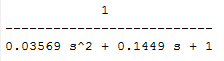
\includegraphics[scale=1.0]{FuncionPlanta}
\renewcommand{\figurename}{Fig.}
\caption{Función de transferencia de la Planta.}
\label{Función de transferencia de la Planta.}
\end{figure}

Primero se debe definir un vector con los coeficientes del numerador y otro con los coeficientes del denominador. Los vectores deben empezar por el coeficiente que multiplica a \textit{s} con mayor exponente hasta llegar al coeficiente que multiplica a \textit{s} con potencia cero, es decir el que no multiplica a ningún \textit{s}. Si al polinomio de \textit{s} le hace falta alguna potencia de \textit{s} quiere decir que el coeficiente para esa potencia de \textit{s} es igual a cero. Por ejemplo, el vector de coeficientes para el polinomio $s^{4}+2s^{2}+s$ debe ser $[1 0 2 1 0]$.  Entonces la definición de la planta mencionada quedaría como sigue: \\

\begin{center}
$num=[1];$ \\
$den=[0.03569  0.1449  1];$ \\
$G=tf(num,den);$ \\
\end{center}

Al ejecutar estos comandos se crea en el \textit{Workspace} de Matlab una función de transferencia de la planta con el nombre \textit{"G"}, debido a que \textit{G} fue el nombre que le fua easignado al ejecutar la función \textit{"tf"}. Ahora se procede a ejecutar \textit{sisotool}, si no se había realizado con anterioridad. Ejecutamos \textit{"sisotool"} en la linea de comandos de MATLAB y se abriran dos ventanas. Una se llama \textit{"Control and Estimation Tool Manager"} y la otra \textit{"SISO design for SISO Design Task"}. A continuación se muestran imágenes de las ventanas emergentes. Si no se abren ventanas parecidas a estas, probablemente este utilizando una versión antigua de \textit{Sisotool}. \\

\begin{figure}[h]
\centering
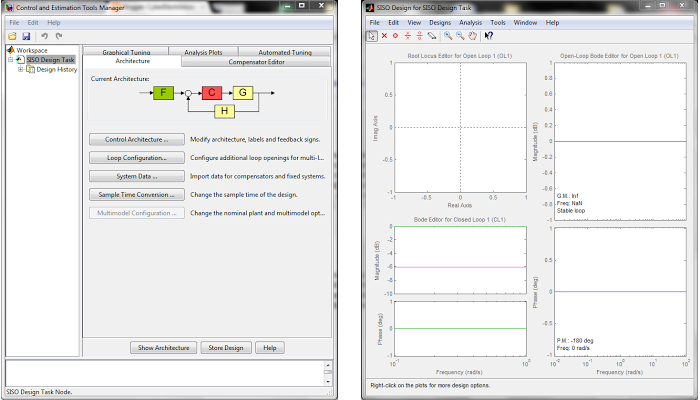
\includegraphics[scale=0.5]{Ventana1}
\renewcommand{\figurename}{Fig.}
\caption{(a) Control and Estimation Tool Manager. (b) SISO design for SISO Design Task.}
\label{Control and Estimation Tool Manager.}
\end{figure}

En \textit{“Control and Estimation Tool Manager”} se escoge la arquitectura de control a utilizar. En la pestaña \textit{“Architecture”}, al dar clic en el botón \textit{“Control Achitecture”} se despliega una ventana que muestra una lista de las arquitecturas disponibles. Para este ejemplo se ha seleccionado la primera de la lista, que se muestra en la \textit{Figura 2.8}. \\

\begin{figure}[h]
\centering
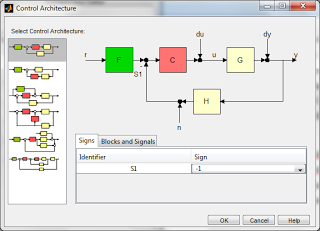
\includegraphics[scale=0.7]{Ventana2}
\renewcommand{\figurename}{Fig.}
\caption{Control Architecture.}
\label{Control Architecture.}
\end{figure}

Después de seleccionar la arquitectura, se importa la función de transferencia de $G(s)$ desde la ventana \textit{“SISO Desing for SISO Desing Task”},  con la opción \textit{“importar”} del menú \textit{“File”}. AL dar clic en \textit{“importar”} Se despliega una ventana en donde se muestra una lista de los sistemas de la arquitectura seleccionada, en este caso  $G$, $H$, $C$ y $F$ que por defecto tienen el valor de \textit{"1"}. La imagen de esta ventana se muestra en la \textit{Fig. 2.9}. \\

\begin{figure}[h]
\centering
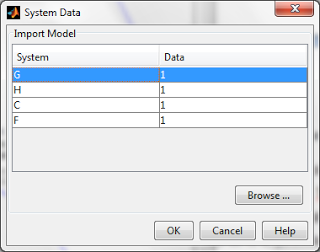
\includegraphics[scale=0.7]{Ventana3}
\renewcommand{\figurename}{Fig.}
\caption{System Data.}
\label{System Data.}
\end{figure}

Se selecciona \textit{“G”} que corresponde a la planta y se presiona \textit{“Browser”}. Entonces aparece otra ventana que muestra una lista de las funciones de transferencia que se encuentran en el \textit{WorkSpace} y en donde debe estar la función \textit{“G”} definida anteriormente y que corresponde a nuestra planta. La imagen de la nueva ventana es la \textit{Fig. 2.10}. \\

\begin{figure}[h]
\centering
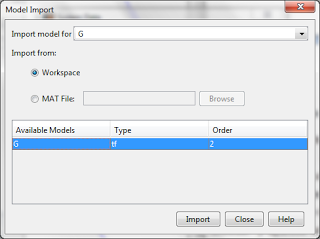
\includegraphics[scale=0.7]{Ventana4}
\renewcommand{\figurename}{Fig.}
\caption{Model Import.}
\label{Model Import.}
\end{figure}

Ahora se selecciona la planta, es decir \textit{“G”}. Se presiona \textit{“import”}, se cierra esta ventana y por último se presiona \textit{“OK”} en la ventana anterior. Habiendo hecho esto, las gráficas de la ventana \textit{"SISO design for SISO Design Task"} debieron modificarse, dicha ventana debe quedar como se observa en la \textit{Fig. 2.11}. \\

\begin{figure}[h]
\centering
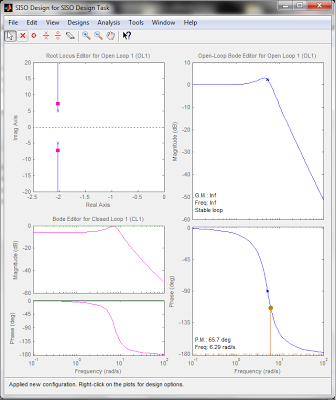
\includegraphics[scale=0.7]{Ventana5}
\renewcommand{\figurename}{Fig.}
\caption{SISO design for SISO Design Task.}
\label{SISO design for SISO Design Task.}
\end{figure}

En la parte superior izquierda de esta ventana se observa la gráfica del $LGR$. Las lineas azules de esta gráfica son el $LGR$ y los puntos rosados representan   la posición actual de los polos del sistema a lazo cerrado. En la arquitectura que se escogió y en general \textit{"C"} es el compensador, y es este sobre el que se enfoca el diseño. Es decir, se necesita encontrar un compensador que haga que el sistema funcione como se desea. \\

Uno de los parametros principales como punto de partida es la definición de la meta a lograr con el control. Para este ejemplo se busca mejorar la respuesta transitoria del sistema, es decir la respuesta del sistema a un escalón. En primer lugar debemos conocer la respuesta del sistema a lazo abierto, es decir de la planta. Para esto utilizamos la herramienta \textit{“Response to step command”} de \textit{sisotool} que se encuentra en el menú \textit{"Analysis"} de la ventana  \textit{"SISO design for SISO Design Task"}. Al ejecutarlo se abre una ventana en la cual aparecen dos gráficas. Esta ventana se muestra en la \textit{Fig. 2.12}. \\

\begin{figure}[h]
\centering
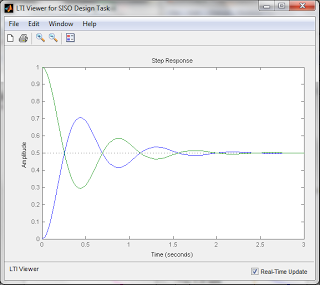
\includegraphics[scale=0.7]{Ventana6}
\renewcommand{\figurename}{Fig.}
\caption{LTI Viewer for SISO Design Task.}
\label{LTI Viewer for SISO Design Task.}
\end{figure}

La gráfica de color Azul es la respuesta del sistema a lazo cerrado y la gráfica de color verde es la señal de salida del compensador. Para ver la respuesta de la planta se da un clic derecho sobre la gráfica, se selecciona \textit{"Systems"} y después \textit{"PlantG"}. Así como se muestra en la \textit{Fig. 2.13}. \\

\begin{figure}[h]
\centering
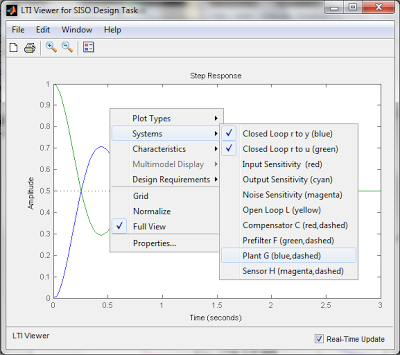
\includegraphics[scale=0.6]{Ventana7}
\renewcommand{\figurename}{Fig.}
\caption{LTI Viewer for SISO Design Task.}
\label{LTI Viewer for SISO Design Task.}
\end{figure}

Entonces aparece una tercera gráfica, de color azul pero con una linea discontinua. Esta es la respuesta transitoria de nuestra planta y nos sirve como referencia para determinar si la respuesta transitoria del sistema a lazo cerrado ha mejorado o no. \\

\begin{figure}[h]
\centering
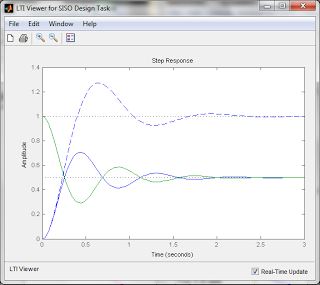
\includegraphics[scale=0.7]{Ventana8}
\renewcommand{\figurename}{Fig.}
\caption{LTI Viewer for SISO Design Task.}
\label{LTI Viewer for SISO Design Task.}
\end{figure}

Ahora regresamos a la ventana de trabajo, la ventana en donde aparece el $LGR$. Los puntos rosados en el $LGR$ representan la posición actual de los polos del sistema a laso cerrado. Estos puntos solo pueden estar sobre la linea de color azul, es decir sobre el $LGR$. Por lo que si se desea poner los polos en una determinada posición, el $LGR$ debe pasar por ahí. Lo anterior es muy importante, mas adelante se explica el por que. \\

Ahora se procede a determinar en donde se deben poner los polos para obtener la respuesta deseada. Pues bien, para solucionarlo \textit{Sisotool} ofrece la posibilidad de incluir algunos requerimientos de diseño en la gráfica del $LGR$. Esto quiero decir que al especificar los requerimientos del diseño, \textit{sisotool} traza una gráfica sobre el $LGR$ que proporciona una idea de donde deben estar los polos para que el sistema funcione como se desea. A continuación se procede a definir que polos deben estar en los puntos que indica \textit{sisotool}, deben ser los polos dominantes. \\

Los polos dominantes son aquellos que más intervienen en la respuesta de un sistema. Aunque la respuesta de un sistema no está completamente determinada por los polos dominantes, puede hallarse una muy buena aproximación de esta hallando la respuesta solo a partir de la contribución de estos polos. Como regla general se toman como polos dominantes aquellos que están más cerca al origen, pues son los que más influyen en la respuesta. \\

Ahora se agregan los requerimientos del diseño. Para este ejemplo se agregan dos requerimientos de diseño: el tiempo de asentamiento o \textit{"Settling time"} y el porcentaje de sobrepaso o \textit{"Percent Overshoot"}. Para agregar un nuevo requerimiento de diseño se da un clic derecho sobre la gráfica del $LGR$ y se selecciona \textit{"Design Requirements"} y luego \textit{"New"}. Así como se muestra en la \textit{Fig. 2.15}. \\

\begin{figure}[h]
\centering
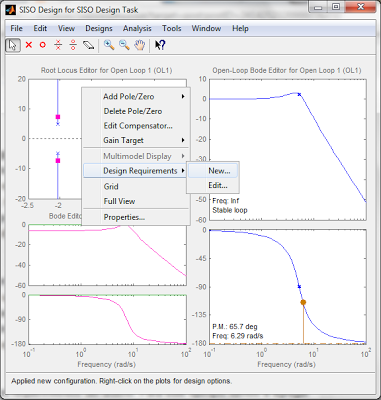
\includegraphics[scale=0.6]{Ventana9}
\renewcommand{\figurename}{Fig.}
\caption{LTI Viewer for SISO Design Task.}
\label{LTI Viewer for SISO Design Task.}
\end{figure}

Los requerimientos que se van a agregar son:

\begin{center}
Settling time = 0.75 \\
Percent Overshoot = 5 \\
\end{center}

Despues de agregar estos requerimientos de diseño la gráfica del LGR queda como se observa en la \textit{Fig. 2.16} \\

\begin{figure}[h]
\centering
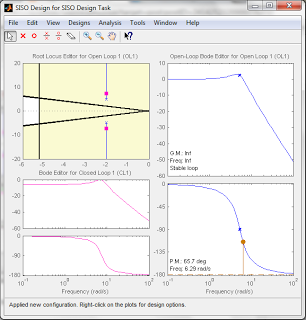
\includegraphics[scale=0.6]{Ventana10}
\renewcommand{\figurename}{Fig.}
\caption{LTI Viewer for SISO Design Task.}
\label{LTI Viewer for SISO Design Task.}
\end{figure}

Al agregar el \textit{“Settling time”} se dibuja una línea vertical  y al agregar el \textit{“Percent Overshoot”} se dibujan dos líneas simétricas sobre el eje real que parten desde el origen con un determinado Angulo y que interceptan la línea dibujada por el \textit{“Settling time”}. Entonces para que se cumplan los requerimientos del diseño los polos dominantes del sistema se deben encontrar en estos puntos de intersección o muy cerca de ellos. Se observa que deben moverse los polos hacia estos puntos, ya que la linea del $LGR$ no pasa por ahí. \\

El proceso de diseño del compensador mediante el método $LGR$ consiste en agregar polos o ceros al compensador para modificar el $LGR$ de tal forma que este pase por los puntos determinados en donde deben estar los polos dominantes para obtener la respuesta deseada. Después de consiguir lo anterior, se arrastran los polos  hasta estos puntos, y entonces la gráfica de la respuesta del sistema debe coincidir con la respuesta deseada. Pero puede que esto no ocurra, y seguramente se debe a que los polos que se ubican en estos puntos no son los dominantes. \\

Para poder predecir los cambios que sufre el $LGR$ al agregar un polo o un cero se debe tener un buen conocimiento de la forma en que se dibuja el $LGR$. Si no se posee este conocimiento se recomienda leer las secciones $6.1$, $6.2$ y $6.3$ del capitulo 6 del libro \textit{Ingeniería de Control Moderna de Ogata}. Las opciones para agregar o quitar polos o ceros están donde indica la \textit{Fig. 2.17}. \\

\begin{figure}[h]
\centering
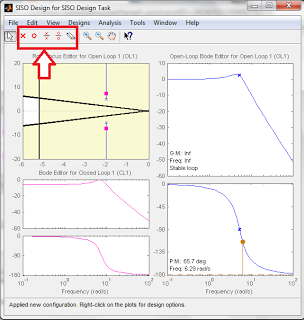
\includegraphics[scale=0.7]{Ventana11}
\renewcommand{\figurename}{Fig.}
\caption{LTI Viewer for SISO Design Task.}
\label{LTI Viewer for SISO Design Task.}
\end{figure}

Se procede a comenzar con el diseño. Para correr los polos hacia la izquierda se agrega un cero en el eje real. Se mueve este cero hasta que el $LGR$ pase por los puntos indicados y se arrastran los polos hasta estos puntos. Despues de hacer esto la gráfica del $LGR$ ha debido quedar como en la \textit{Fig. 2.18}. \\

\begin{figure}[h]
\centering
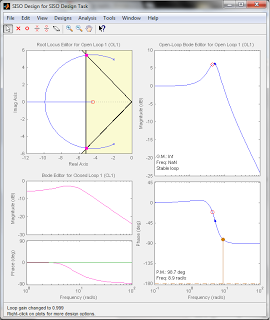
\includegraphics[scale=0.7]{Ventana12}
\renewcommand{\figurename}{Fig.}
\caption{LTI Viewer for SISO Design Task.}
\label{LTI Viewer for SISO Design Task.}
\end{figure}

Y la gráfica de la respuesta del sistema que se muestra con la linea azul contínua ha debido quedar como sigue. \\

\begin{figure}[h]
\centering
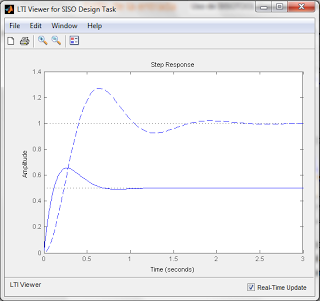
\includegraphics[scale=0.6]{Ventana13}
\renewcommand{\figurename}{Fig.}
\caption{LTI Viewer for SISO Design Task.}
\label{LTI Viewer for SISO Design Task.}
\end{figure}

En esta imagen se puede apreciar que efectivamente  el tiempo de asentamiento de la respuesta del sistema a lazo cerrado ahora se encuentra alrededor se $0.75 segundos$. Aunque no es tan claro que se halla cumplido con el requerimiento del porcentaje de sobrepaso. Como se dijo antes al especificar los requerimientos del diseño, \textit{sisotool} traza una gráfica  sobre el $LGR$ que proporciona una idea de donde deben estar los polos para que el sistema funcione como se desea. Es decir solo da una aproximación. \\

Ya se logro cumplir con el requerimiento de tiempo de asentamiento pero se genero otro problema y es el gran error en estado estacionario que posee ahora el sistema a lazo cerrado. La salida debe asentarse en un valor de $1$ pero lo hace en un valor aproximado de $0.45$. Ahora para corregir el error en estado estacionario se agrega un integrador, es decir un polo en el origen. El $LGR$ y la gráfica de la respuesta del sistema se observan en la \textit{Fig. 2.20}. \\

\begin{figure}[h]
\centering
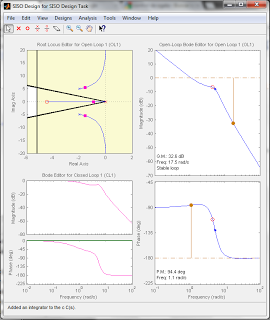
\includegraphics[scale=0.7]{Ventana14}
\renewcommand{\figurename}{Fig.}
\caption{LTI Viewer for SISO Design Task.}
\label{LTI Viewer for SISO Design Task.}
\end{figure}

Tal como se ve, ahora no hay error en estado estacionario pero todo lo demás se altero y la gráfica del $LGR$ se modifico totalmente. La gráfica del $LGR$ puede restablecerse a forma parecida a la anterior agregando un cero en el eje real entre el cero que se había agregado antes y el polo en el origen que se agregó ahora, ya que esto obliga a que la parte del $LGR$ que empieza desde el polo en el origen llegue solo hasta el nuevo cero que se agregó. Haciendo esto que los polos complejos conjugados que existían originalmente vuelvan a interactuar de la misma forma que antes con el primer cero que se agregó. Al agregar el nuevo cero el $LGR$ queda como se observa en la \textit{Fig. 2.21}. \\

Como ahora el polo que esta mas cerca al origen fue el que se agregó, los otros dos polos complejos conjugados no son los dominantes, por lo que las gráficas de los requerimientos de diseño ya no son proporcionan confiabilidad. \\

\begin{figure}[h]
\centering
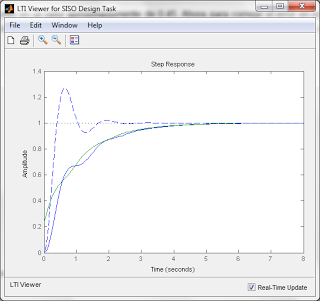
\includegraphics[scale=0.7]{Ventana15}
\renewcommand{\figurename}{Fig.}
\caption{LTI Viewer for SISO Design Task.}
\label{LTI Viewer for SISO Design Task.}
\end{figure}

Como regla general un sistema es mas estable entre más alejados del origen se encuentren sus polos. Así que se corren los polos a la izquierda para ver el resultado. \\

Mientras se mueven los polos hacia la izquierda se llega un punto en el que se obtiene la siguiente gráfica de la \textit{Fig. 2.22} con la respuesta del sistema. \\

\begin{figure}[h]
\centering
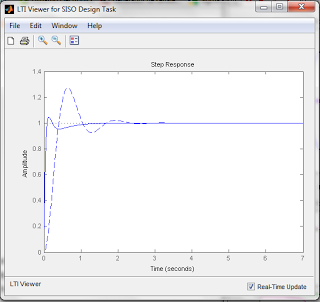
\includegraphics[scale=0.6]{Ventana16}
\renewcommand{\figurename}{Fig.}
\caption{LTI Viewer for SISO Design Task.}
\label{LTI Viewer for SISO Design Task.}
\end{figure}

Como se observa, esta respuesta es bastante mejor de lo que se tenia plantedo inicialmente, pero también pueden ocurrir el caso en que no se logra llegar siquiera a los objetivos planteados inicialmente. Si se siguen moviendo los polos a la izquierda la respuesta seguirá mejorando, pero cuando se hace eso se esta aumentando la ganancia del compensador, y no se podrá implementar un compensador que tenga una ganancia muy elevada. Para ver como queda función de transferencia del compensador se selecciona la opción $"edit$ $compensator"$ del menú \textit{"designs"} y se abre una ventana donde se muestra la ecuación del compensador que se debe utilizar para conseguir la respuesta a la que se ha llegado. Tal como en la \textit{Fig. 2.23}. \\

\begin{figure}[h]
\centering
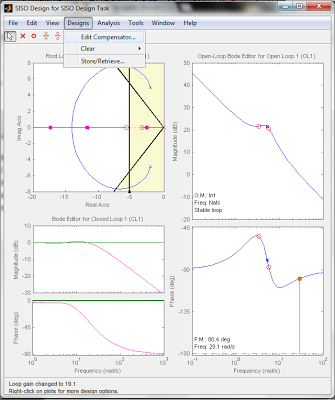
\includegraphics[scale=0.7]{Ventana18}
\renewcommand{\figurename}{Fig.}
\caption{LTI Viewer for SISO Design Task.}
\label{LTI Viewer for SISO Design Task.}
\end{figure}

\newpage





% ==============================================================================================
%									CAPITULO DISEÑO METODOLÓGICO
% ==============================================================================================

\chapter{Diseño Metodologico}

%\section{Analisis}

%\section{Delimitaciones}



\section{Primera Etapa - Tanque Independiente}

La figura ----- muestra el diseño del sistema de entrenamiento de tanques acoplados M-ECCI. El sistema cuenta con dos tanques ubicados en la sección superior del sistema. cada tanque cuenta con un sensor de nivel para determinar la altura del líquido y con un desfogue hacia el tanque de reserva mediante válvulas
ubicadas en el ducto de salida de cada tanque. \\

Además el sistema cuenta con un tanque de reserva, el mismo que proporciona el líquido a ser bombeado hacia los tanques superiores. En la sección inferior se encuentra ubicada una bomba encargada de distribuir el liquido desde el tanque de reserva hacia los demas. \\

El problema se centra en la obtención del comportamiento de nivel del líquido a través del tiempo $t$ de un tanque, dado el flujo de entrada $q_{i}(t)$. Se asume que el flujo de salida del tanque es una función lineal de la altura de líquido en su interior ($q_{o}=k*h$) y que el tanque tiene un área de sección transversal constante. Se asume también que la densidad y el flujo de entrada $q_{i}(t)$ son constantes.

\subsection{Modelo Dinamico Planta M-ECCI}

Se toma la ecuación inicial (5.1) para determinar la variación de nivel del tanque teniendo en cuenta los caudales de entrada y salida, así como el área del tanque, la cual se considera constante.

\begin{equation}
A\frac {dh\left( t\right) }{dt}=q_{i}-q_{o}
\end{equation}

El caudal de salida $q_{o}$ se a continuación.

\begin{equation}
q_{o}=\frac{h}{R}
\end{equation}

Se reemplaza (5.1) en (5.2) y se obtiene la ecuación (5.3) para realizar el despeje de la variable a controlar, el nivel del tanque.

\begin{equation}
A\frac {dh\left( t\right) }{dt}=q_{i}-\frac {h}{R}
\end{equation}

Se debe tener en cuenta que $h$ y $q_{i}$ son variables dependientes del tiempo $(t)$, por tanto se tiene que:

\begin{equation}
\frac {dh\left( t\right) }{dt}=\frac {q_{i}(t)-\frac {h(t)}{R}}{A}
\end{equation}

Se opera la ecuación (5.4) para obtener (5.5), una ecuación simplificada.

\begin{equation}
\frac {dh\left( t\right) }{dt}=\frac {Rq_{i}(t)-h(t)}{AR}
\end{equation}

%Evaluando en estado estable, $t=0$

%\begin{equation}
%\frac {d\overline {h\left( 0\right) }}{dt}=\frac {R\overline {q_{i}\left( 0\right) }-\overline {h\left( o\right) }}{AR}
%\end{equation}

%Operando (resta) (4)-(5) de las variables

%\begin{equation}
%\end{equation}

%\begin{equation}
%ARd\frac {\left[ h\left( t\right) -\overline {h\left( 0\right) }\right] }{dt}=R\left[ q_{i}\left( t\right) -\overline {q_{i}\left( 0\right) }\right] -\left[ h\left( t\right) -\overline {h\left( 0\right) }\right]
%\end{equation}

%Realizando cambio de variable

%\begin{equation}
%Q_{in}=q_{i}\left( t\right) -\overline {q_{i}\left( 0\right) }
%\end{equation}

%\begin{equation}
%H=h\left( t\right) -\overline {h\left( 0\right) }
%\end{equation}

%\begin{equation}
%A\frac {RdH}{dt}=RQ_{in}\left( t\right) -H\left( t\right)
%\end{equation}

En (5.6), se despeja las variable de nivel a un lado de la ecuación a fin de factorizar.

\begin{equation}
A\frac {Rdh}{dt}+h\left( t\right) =Rq_{i}\left( t\right)
\end{equation}

Se tiene que $AR$ corresponde a la base de tiempo de la ecuación y $R$ la resistencia que opone la válvula al paso del fluido, sin embargo, este factor es cambiante dependiendo del elemento que se esté usando.

\begin{center}
$\tau =AR$ \\
$K=R$
\end{center}

Se reemplazan los valores anteriores en la ecuación (5.6), de modo que se obtiene:

\begin{equation}
\frac {\tau dh}{dt}+h\left( t\right) =Kq_{i}\left( t\right)
\end{equation}

Se aplica transformada de Laplace para derivada de primer orden en la ecuación (5.7).

\begin{equation}
\tau sh\left( s\right) +h\left( s\right) =Kq_{i}\left( s\right)
\end{equation}

Se factorizan los terminos de altura \textit{h}.

\begin{equation}
h\left( s\right) \left( \tau s+1\right) =Kq_{i}\left( s\right)
\end{equation}

$h(s)$ equivale a la salida del sistema y $q_{i}(s)$ a la entrada. Ya que el modelo de función de transferencia es $G=out/in$, se tiene que:

\begin{equation}
\frac {h\left( s\right) }{q_{i}\left( s\right) }=\frac {K}{\tau s+1}
\end{equation}

La ecuación (5.10) representa el modelo de función de transferencia de primer orden para la planta. \\

Para realizar el modelo especifico del tanque, es necesario realizar el cambio de variable inverso a la ecuación (5.7) aplicando la ecuación (5.10).

\begin{equation}
\frac {h\left( s\right) }{q_{i}\left( s\right) }=\frac {R}{AR+1}
\end{equation}

\subsection{Linealización}

Sin importar que geometría posea un tanque, el caudal a través de la válvula de salida será proporcional a la raíz cuadrada del nivel del líquido directamente sobre la válvula. De este modo el caudal de salida del tanque $q_{o}$, será (5.12):

\begin{equation}
q_{o}=C\sqrt{h}
\end{equation}

Donde $C$ es la constante que involucra el coeficiente de la válvula y que además esta relacionado con la apertura de la misma y $h$ el nivel de líquido en el tanque. \\

De este modo tenemos que el modelo del proceso de nivel en un tanque, dado por la ecuación (5.1) puede expresarce con en la siguiente ecuación.

\begin{equation}
A\frac{dh}{dt}=q_{i}-C\sqrt{h}
\end{equation}

Donde $A$ es área del tanque y $q_{i}$ es el flujo de entrada de líquido al tanque. \\

El primer término de la ecuación (5.13) representa el diferencial de caudal en el tanque, considerando que el área del tanque es uniforme, es decir se mantiene constante, a lo largo de todo el tanque. Observando esta ecuación es posible definir que el modelo representa a un proceso no lineal. La no linealidad se debe a la presencia del término de raíz cuadrada en la ecuación. Una opción para poder trabajar con este modelo es linealizar el término no lineal de dicha ecuación. La función no lineal queda definida en la ecuación (5.14).

\begin{equation}
f(h)=\sqrt{h}
\end{equation}

En este punto, no es posible realizar el procedimiento realizado en la seccion anterior, y aplicar la transformada de Laplace. Esto es debido a la presencia del termino no lineal para el cual no hay transformada simple. Por medio de la expansión en serie de Taylor, la función puede ser expandida alrededor del punto en estado estacionario $hs$, Asi.

\begin{equation}
\sqrt{h}=hs^{\frac{1}{2}}+\frac{1}{2}hs^{\frac{-1}{2}}(h-hs)
\end{equation}

Donde $hs$ es el valor de $h$ en estado estable. \\

Entonces reemplazando la ecuación (5.15) en la ecuación (5.13) se obtiene:

\begin{equation}
A\frac{dh}{dt}=q_{i}-C\left[hs^{\frac{1}{2}}+\frac{1}{2} hs^{-\frac{1}{2}}\left(h-hs\right) \right]
\end{equation}

Así en la ecuación (5.16) se tiene la ecuación del modelo de nivel del tanque linealizada en un punto de estado estable $hs$. Ahora se procede a definir la variable $y=(h–hs)$ e introducir la variable $u=(q_{i}–q_{i}s)$, donde $q_{i}s$ representa el valor de caudal de entrada en estado estable. \\

Adicionalmente se debe recordar que en estado estable $dh/dt=0$, entonces aplicando esta condición a la ecuación (5.13) se obtiene:

\begin{equation}
q_{i}s=C\sqrt{hs}
\end{equation}

De este modo la ecuación (5.16) se convierte en:

\begin{equation}
\tau\frac{dy}{dt}=Ku-y
\end{equation}

Donde se define los valores de las constantes $\tau$ y $K$ como sigue a continuación:

\begin{equation}
\tau=A\frac{2(hs)^{\frac{1}{2}}}{C}
\end{equation}

\begin{equation}
K=\frac{2(hs)^{\frac{1}{2}}}{C}
\end{equation}

La constante $\tau$ es denominada constante de tiempo mientras que la constante $K$ es la ganancia de estado estable. Aplicando a la ecuación (5.18) la transformada de La Place se obtiene la función de transferencia (5.21), la cual representa teóricamente el modelo del nivel del tanque en un punto de estado estable $hs$.

\begin{equation}
y(s)=\frac{K}{\tau s+1}u(s)
\end{equation}

Se debe recordar que la ecuación (5.21) es valida solo para el punto de estabilización $hs$, para un nuevo punto de estabilización $hs_{2}$ los valores de las constantes $\tau$ y $K$ serán diferentes.




\subsection{Calculo de Parametros}

En este punto se realiza el cálculo para el valor de la constante de tiempo, $\tau$. Considerando un valor de estado estable $hs$ de 40cm y conociendo el área del tanque 1 el cual es -------. El valor de la constante $C$ es desconocido ya que depende de las características de la válvula colocada a la salida del tanque. Sin embargo es posible hallar el valor de dicha constante experimentalmente y calcular un valor aproximado de $\tau$. El procedimiento que se lleva a cabo se presenta a continuación. \\

Es necesario conocer el caudal a la salida de la válvula conectada a la parte inferior del tanque. La primera limitación de este procedimiento es
que no se dispone de un medidor de caudal ubicado directamente después de la válvula. Para solucionar este problema se toman las mediciones del medidor de caudal bicado en la tubería de entrada de líquido, figura 3.3. Se debe tener en cuenta que en estado estable el caudal de entrada es equivalente al caudal de salida, por lo tanto, una vez que se alcance el estado estable el caudal medido a la entrada será igual al caudal que
existe a la salida del tanque. \\

Conociendo las dimensiones reales de la tubería, se procede a realizar una verificación inicial sobre los cálculos ideales para los caudales de entrada y salida del tanque.

\begin{center}
Tuberia de entrada = 1/2 pulgada \\
Tuberia de salida = 1/4 pulgada
\end{center}

El caudal máximo que atraviesa una sección de tubería esta dado por la ecuación de continuidad:

\begin{equation}
Q=\upsilon A=\frac{4\upsilon}{\pi D^{2}}
\end{equation}

Donde $Q$ es el caudal volumétrico o flujo de agua que circula por la tubería $(m^{3}/s)$, $\upsilon$ es la velocidad del agua en el interior de la tubería $(m/s)$, $A$ es el area de la sección transversal de la tuberia $(m^{2})$ y $D$ es el diámetro de la misma. Debido a que la tubería posee forma circular, el área esta dada por:

\begin{equation}
A=\pi r^{2}
\end{equation}

El diámetro exterior de un tubo de PVC de 1/2 pulgada no es exacto, como se puede observar en la Figura -----, siendo realmente de 0.840 pulgadas (2.1336cm). Para obtener valores con mayor exactitud, se debe partir del diámetro interno de la tubería, obteniendo así una medida de 0.9cm para la tuberia de entrada y --cm para la tubería de salida.

\begin{figure}[h]
\centering
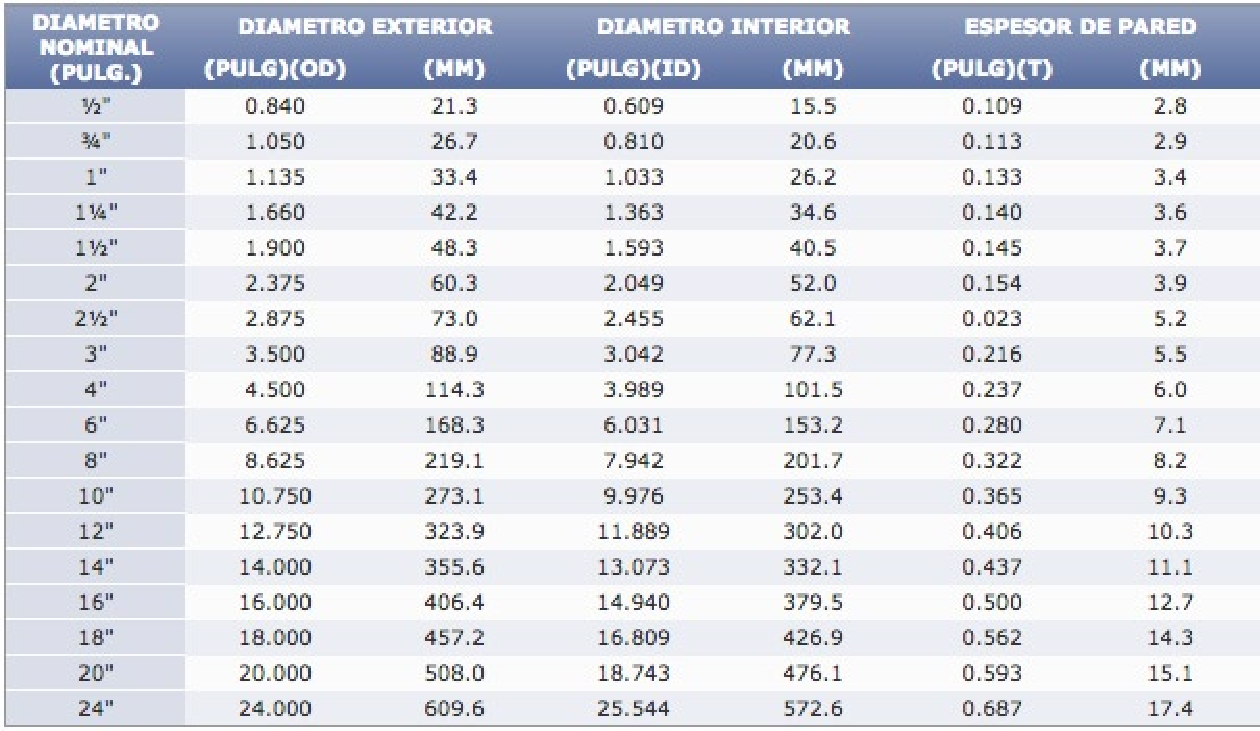
\includegraphics[scale=0.5]{DiametrosPVC}
\renewcommand{\figurename}{Fig.}
\caption{Diametros nomiales de tuberia PVC.}
\label{Diametros nomiales de tuberia PVC.}
\end{figure}

Para tuberias plasticas y con flujo laminar, la velocidad promedio del agua es de 2 m/s. Usando la eciación ------ se obtiene un caudal de --- para la tuberia de entrada y uno de ---- para la de salida. \\ 

En este punto se presenta la segunda limitación, ya que el caudal maximo de entrada sobrepasa al de salida, lo que indica que el volumen de liquido que ingresa al tanque es muy superior, impidiendo alcanzar un punto de estabilización. En pruebas reales de verificación sobre la planta, se llega a la conclusión de limitar la velocidad de operación de la bomba que alimenta el tanque, para que de esta manera el caudal de entrada no sobrepase al de salida y garantizar el estado estable. \\


 





\subsection{Diseño de Controlador}

El objetivo de llevar a cabo el modelamiento y linealización de la planta en las secciones anteriores es específicamente diseñar un controlador para la misma. El controlador es seleccionado de la familia de controladores PID, de la cual se pretende adoptar la mejor combinación, que cumpla los requerimientos establecidos. La familia de controladores PID pertenece a los métodos clásicos de control, sin embargo, existen muchos tipos de configuraciones de controladores que pueden ser estudiados y aplicados a partir del modelo ya obtenido. \\

%Esta seccion se enfoca en el modelo linealizado de la planta y se parte de este para diseñar un controlador que se ajuste a los requerimientos detallados mas adelante. Se desarrolla la implementación de dicho controlador haciendo uso del conjunto de herramientas PID de LabVIEW, el cual posee las funciones básicas relacionadas con el uso de controladores PID. \\

Básicamente, usando el modelo de la planta linealizada se encuentran los parámetros de un controlador de la familia PID para la misma, y se evaluan los resultados de las simulaciones.




\section{Segunda Etapa - Tanques Acoplados}

En base al desarrollo llevado a cabo en la primera etapa, se amplia el alcance del sistema, permitiendo analizar el comportamiento de un segundo tanque, mas especificamente el tercero, el cual se encuentra ubicado en la zona inferior de la planta y es el encargado de recibir el liquido proveniente del primer tanque. En un escenario real, se hace necesario conocer el comportamiento del nivel sobre ambos tanques, ya que el flujo del liquido en lazo cerrado de la planta real se realiza atravez de ambos y debido a esto no se debe analizar el comportamiento de uno de los tanques obviando la respuesta del segundo. \\

Debido a lo mensionado anteriormente, se procede con el analisis para dos tanques acoplados.

\subsection{Modelo Matematico}

El sistema se encuentra conformado por dos tanques en serie de áreas de sección transversal constantes, por donde fluye un líquido (una sustancia pura) que pasa el primer tanque el segundo tanque como se muestra la figura uno. El objetivo es modelar el sistema para predecir la variación de la altura del segundo tanque de acuerdo a la alimentación del primer tanque $f_{0}(t)$. Se asume que el flujo de salida de cada tanque es una función lineal de la altura de líquido en el respectivo tanque ($f_{1}=K_{1}h_{1}$ y $f_{2}=K_{2}h_{2}$).

%\begin{figure}[h]
%\centering
%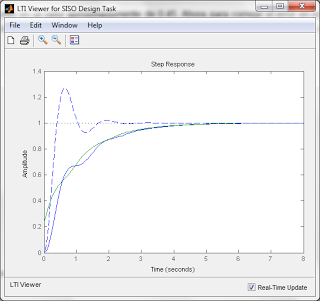
\includegraphics[scale=0.7]{Ventana15}
%\renewcommand{\figurename}{Fig.}
%\caption{LTI Viewer for SISO Design Task.}
%\label{LTI Viewer for SISO Design Task.}
%\end{figure}

Para el desarrollo del modelo matemático se trabajaran dos volúmenes de control como se observa en la figura 2. Cómo se pretende obtener la dinámica del nivel del tanque, entonces debe saber cuál es la acumulación en el tanque, conociendo tambien que esta depende del flujo de entrada y salida en el tanque. La dinamica del primer volumen de control Determinará el flujo de entrada en el segundo tanque, por lo que se hace necesario tomar este primer volumen de control. El segundo volumen de control se plantea para realizar sobre el modelo matemático que termine la dinámica del tanque 2 y así predecir el nivel del tanque.

%\begin{figure}[h]
%\centering
%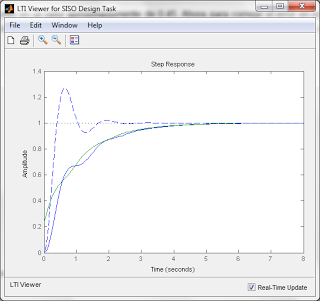
\includegraphics[scale=0.7]{Ventana15}
%\renewcommand{\figurename}{Fig.}
%\caption{LTI Viewer for SISO Design Task.}
%\label{LTI Viewer for SISO Design Task.}
%\end{figure}









%\section{Materiales y Equipos}

%\section{Analisis de Resultados}





% ==============================================================================================
%								CAPITULO CRONOGRAMA DE ACTIVIDADES
% ==============================================================================================

%\chapter{Cronograma de Actividades}

%\section{Evidencias}

%\newpage





% ==============================================================================================
%									CAPITULO CONCLUSIONES
% ==============================================================================================

\chapter{Conclusiones}

A partir de los resultados obtenidos con el presente proyecto de grado, es posible concluir que: \\

\begin{itemize}
\item Se realizó el montaje y la instrumentación electrónica de un sistema de tanques acoplados en el laboratorio de control e instrumentación de la E3T como se puede observar de los resultados presentados en la sección 2.1 (Figura 8), donde se evidencia la configuración del sistema de control implementado constituido por una válvula proporcional DANFOSS, válvulas manuales y de encendido apagado, un trasmisor de presión diferencial HONEYWELL y un controlador universal UDC1200.
\item Se instrumentaron y calibraron tanto el sensor de presión como el actuador (válvula proporcional), para efectuar manipulación del nivel de líquido en el sistema mediante el controlador industrial. Lo anterior se ilustra en las secciones 2.1 y 2.3, en las cuales se explica la caracterización de cada elemento del sistema de control y los respectivos ajustes en los rangos y escalas de sus correspondientes señales.
\item Se realizó un procedimiento experimental para obtener los parámetros de un modelo matemático apropiado para el sistema, tales como resistencias hidráulicas representadas por válvulas manuales y on-off, al igual que capacitancias hidráulicas relacionadas con el área de sección transversal de los tanques. Lo anterior se ilustra en las secciones 3.1 y 3.2, desarrollos a partir de los cuales se obtuvo una representación matemática del comportamiento del sistema a manera de función de transferencia (ecuacion 3.15).
\item Se validó el modelo matemático obtenido con medidas del sistema real mediante una prueba en lazo abierto que consistió en aplicar una entrada escalon al sistema experimental y comparar posteriormente los resultados de su respuesta con los generados numéricamente para el modelo empleando MATLAB®, como se puede observar en la Figura 14 de la seccion 3.3.
\item Se diseñó e implementó un controlador PID en un dispositivo industrial de referencia HONEYWELL UDC1200 para regular el nivel del tanque de salida. Para esto se calcularon y sintonizaron los valores para las constantes del controlador utilizando el primer método de Ziegler \& Nichols. Los resultados obtenidos se muestran en la Tabla 5, las Figuras 19-20 y la sección 4.3, verificando la acción de control y la atenuación del efecto de una perturbación aplicada al sistema mediante la variación del parámetro $R_{1}$. A pesar de ello, la respuesta experimental obtenida difiere de la predicha por la teoría principalmente por la aparición de oscilaciones, lo cual puede deberse a los errores de aproximacion generados por el modelo lineal propuesto para el sistema.
\item Finalmente se implementó una sintonización automática de los parámetros para el controlador UDC1200, demostrando un mejoramiento en la respuesta del sistema controlado tal y como se describe en la sección 4.4.
\end{itemize}






% ==============================================================================================
%									CAPITULO TRABAJO FUTURO
% ==============================================================================================

\chapter{Trabajo Futuro}

En desarrollo del presente proyecto de grado se generaron las inquietudes resumidas a continuacion. \\

\begin{itemize}
\item El sistema real no es un sistema lineal y por tal motivo las variaciones de referencia deben hacerse alrededor del punto de operacion. Asimismo, este valor de referencia no debe superar los 40 cm de altura debido a restricciones practicas.
\item Tomando en cuenta la ubicacion de la tuberia de acople de los dos tanques y la tuberia de desag\"ue, el mínimo nivel de líquido de cada uno de los tanques puede variar entre 1 y 4 cm. Para el caso del tanque de salida es posible disminuir este nivel mínimo desconectando la manguera del sensor de presion.
\item La potencia de salida del controlador se ajusto al 40\%, debido a que es mayor la cantidad de flujo de liquido suministrado al tanque de entrada que el evacuado por la tuberia de acople hacia el tanque de salida, ocasionando que el tanque de entrada se rebase hasta su tope.
\item El valor de perturbacion seleccionado para $R_{1}$ fue la maxima apertura de la valvula, debido a que para otro valor de resistencia el efecto de la perturbacion no era discriminante, ya que el sistema en estado estable presenta oscilaciones.
\end{itemize}

Asi mismo, como trabajos futuros complementarios a este trabajo de grado se plantean. \\

\begin{itemize}
\item La implementacion de un sistema de recirculacion de liquido con el fin de aprovechar mejor el recurso hidrico del proceso.
\item La eleccion o diseño de un sistema de sensado cuyos rangos de operacion estén mas cercanos al valor real del sistema.
\item La implementacion de una accion de control y modelado del sistema en donde se contemple la interaccion de nivel de liquido entre los dos tanques.
\end{itemize}





% ==============================================================================================
%								CAPITULO CRONOGRAMA DE ACTIVIDADES
% ==============================================================================================

%\chapter{Bibliografia}





% ==============================================================================================
%												ANEXOS
% ==============================================================================================


%\appendix

%\chapter{Tarjetas de circuitos impresos}

%\section{Historia}


















%\bibliographystyle{IEEEtran}
%\bibliography{prueba}
%\printbib{RPFCU-HBB}

\end{document}